\documentclass[12pt,draft]{report}
\usepackage{graphicx} % Required for inserting images
\usepackage{multirow}
\usepackage{lscape}
\usepackage{pdflscape}
\usepackage{fixltx2e}
\usepackage{geometry}
\usepackage{wasysym}
\usepackage{amsmath}
\usepackage{amssymb}
\usepackage{caption}
\usepackage{subcaption}


\newcommand{\head}[1]{\textnormal{\textbf{#1}}}
\newcommand\ion[2]{\text{#1\,\textsc{\lowercase{#2}}}}

\title{Thesis Phase-1}
\author{Sameer Patidar}
\date{July 2023}

\begin{document}


\begin{landscape}

\begin{figure}
\centering
\vspace{-20mm}
\hspace*{-35mm}
\captionsetup{oneside,margin={0cm,35mm}}
\includegraphics[width=1.25\linewidth]{System-Plots/3C263_z=0.140756_sys_plot.png}
\end{figure}

\end{landscape}


\begin{center}
 
\begin{tabular}{cccc}
        \hline \hline \tabularnewline
       \head{Ion} & \head{v (km s\textsuperscript{$\mathbf{-1}$})} & \head{b (km s\textsuperscript{$\mathbf{-1}$})} & \head{log [N cm\textsuperscript{$\mathbf{-2}$}]} 
       \tabularnewline \tabularnewline \hline \tabularnewline 

\ion{Si}{iii}  &    -18 $\pm$ 8   &    35 $\pm$ 11    &     12.39 $\pm$ 0.09 \\
\ion{C}{iv}   &    -10 $\pm$ 3   &    33 $\pm$ 0    &     13.71 $\pm$ 0.04 \\
\ion{O}{vi}   &    0 $\pm$ 2   &    26 $\pm$ 4    &     13.63 $\pm$ 0.04 \\
\ion{H}{i}   &    -14 $\pm$ 1   &    87 $\pm$ 10    &     13.49 $\pm$ 0.06 \\
\ion{H}{i}   &    0 $\pm$ 1   &    28 $\pm$ 1    &     14.49 $\pm$ 0.02 \\
\tabularnewline \hline \hline \tabularnewline

\end{tabular}

\end{center}

N(\ion{H}{I})=13.49 \\

Excluding \ion{O}{vi} : $n_H$ = -3.88 $\pm$ 0.04 \hspace{10mm} $Z$ = 1.06 $\pm$ 0.05

Including \ion{O}{vi} : $n_H$ = -4.13 $\pm$ 0.02 \hspace{10mm} $Z$ = 0.99 $\pm$ 0.04
\\\\
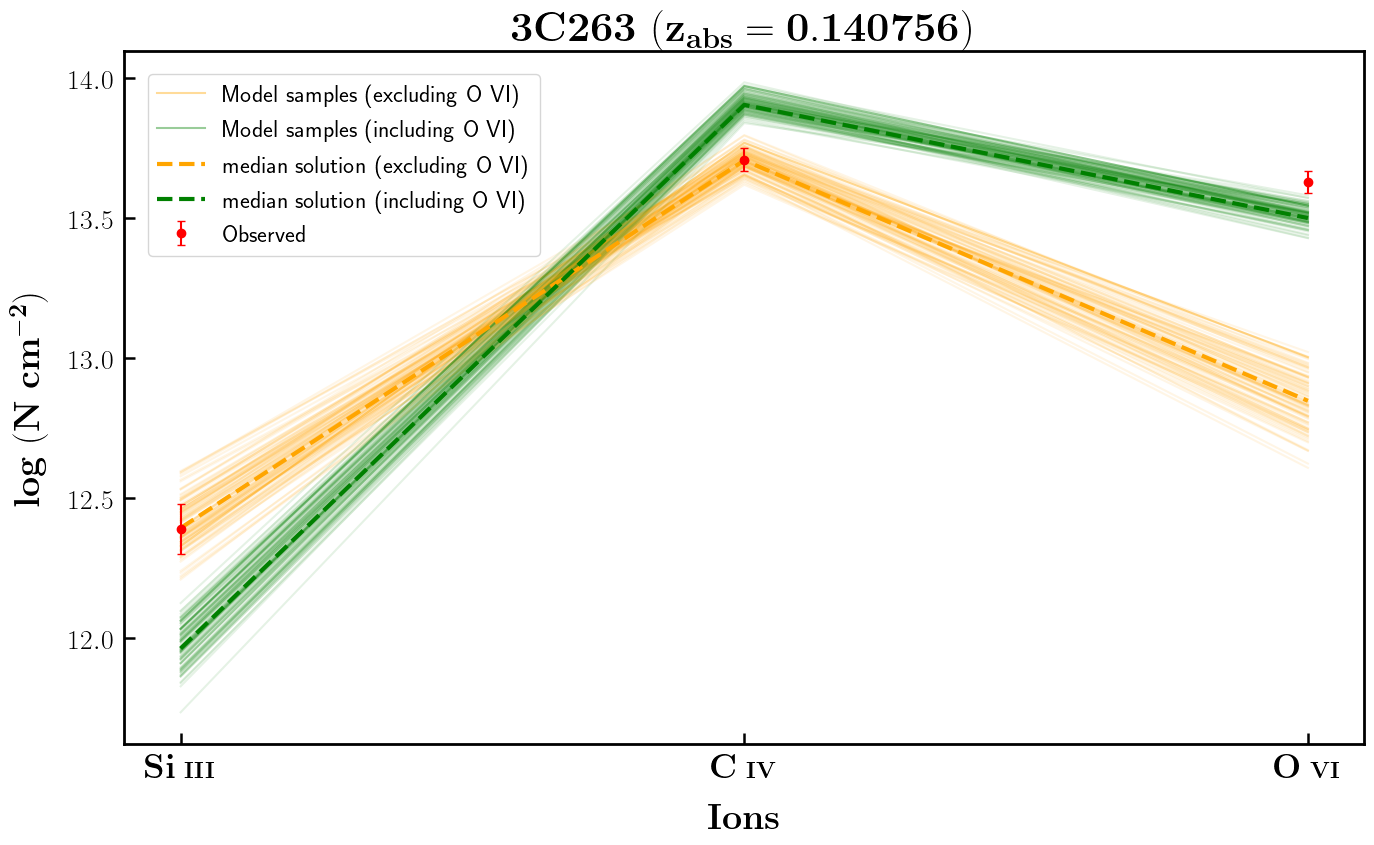
\includegraphics[width=1\linewidth]{Ionisation-Modelling-Plots/3c263-z=0.140756-compI.png}


\newpage


\begin{landscape}

    \begin{figure}
    \centering
    \vspace{-20mm}
    \hspace*{-35mm}
    \captionsetup{oneside,margin={0cm,35mm}}
    \includegraphics[width=1.25\linewidth]{System-Plots/PKS0637-752_z=0.161064_sys_plot.png}
    \end{figure}
    
\end{landscape}


\begin{center}
 
    \begin{tabular}{cccc}
            \hline \hline \tabularnewline
           \head{Ion} & \head{v (km s\textsuperscript{$\mathbf{-1}$})} & \head{b (km s\textsuperscript{$\mathbf{-1}$})} & \head{log [N cm\textsuperscript{$\mathbf{-2}$}]} 
           \tabularnewline \tabularnewline \hline \tabularnewline 
    
           \ion{N}{v}   &    -42 $\pm$ 6    &    40 $\pm$ 9    &     13.37 $\pm$ 0.07 \\
           \ion{Si}{iii}   &    11 $\pm$ 4    &    30 $\pm$ 7    &     12.37 $\pm$ 0.06 \\
           \ion{O}{vi}   &    0 $\pm$ 3    &    48 $\pm$ 5    &     14.02 $\pm$ 0.03 \\
           \ion{H}{i}   &    -13 $\pm$ 2    &    162 $\pm$ 21    &     13.6 $\pm$ 0.06 \\
           \ion{H}{i}   &    -1 $\pm$ 1    &    45 $\pm$ 1    &     15.01 $\pm$ 0.02 \\
    \tabularnewline \hline \hline \tabularnewline
    
    \end{tabular}
    
    \end{center}
    
    N(\ion{H}{I})=13.60 \\
    
    Excluding \ion{O}{vi} : $n_H$ = -4.05 $\pm$ 0.03 \hspace{10mm} $Z$ = 1.20 $\pm$ 0.05
    
    Including \ion{O}{vi} : $n_H$ = -4.12 $\pm$ 0.01 \hspace{10mm} $Z$ = 1.30 $\pm$ 0.04
    \\\\
    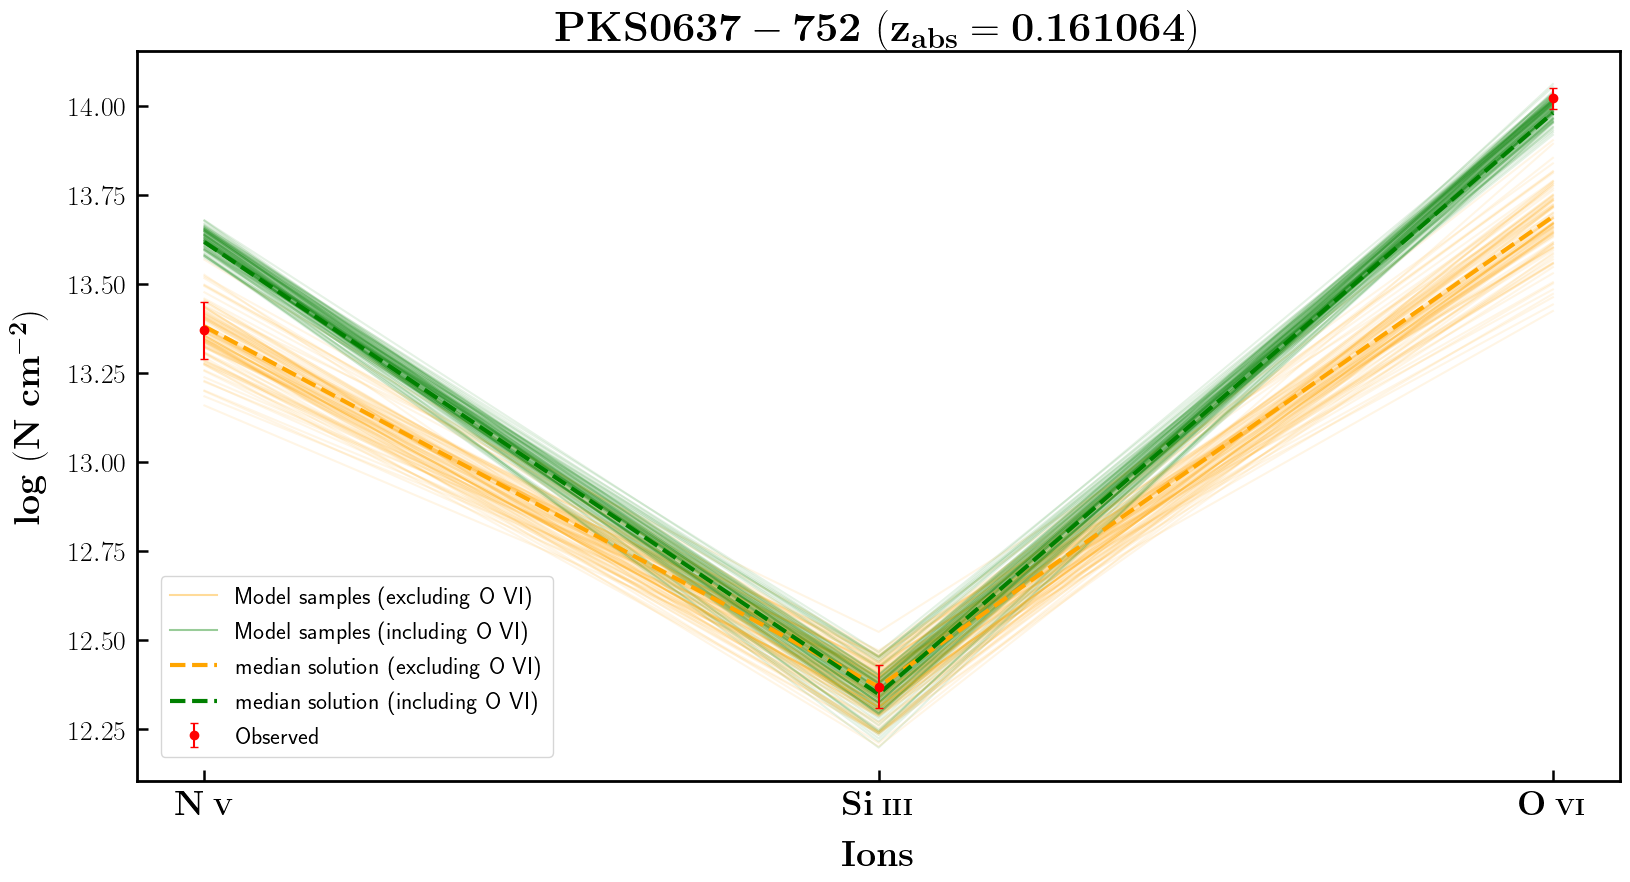
\includegraphics[width=1\linewidth]{Ionisation-Modelling-Plots/pks0637-z=0.161064-compI.png}



\newpage


\begin{landscape}

    \begin{figure}
    \centering
    \vspace{-20mm}
    \hspace*{-35mm}
    \captionsetup{oneside,margin={0cm,35mm}}
    \includegraphics[width=1.25\linewidth]{System-Plots/PKS0637-752_z=0.417539_sys_plot.png}
    \end{figure}
    
\end{landscape}


\begin{center}
    
    \begin{tabular}{cccc}
        \hline \hline \tabularnewline
        \head{Ion} & \head{v (km s\textsuperscript{$\mathbf{-1}$})} & \head{b (km s\textsuperscript{$\mathbf{-1}$})} & \head{log [N cm\textsuperscript{$\mathbf{-2}$}]} 
        \tabularnewline \tabularnewline \hline \tabularnewline 
    
        \ion{Si}{iii}   &    -5 $\pm$ 4    &    35 $\pm$ 7    &     12.74 $\pm$ 0.06 \\
        \ion{C}{iii}   &    -4 $\pm$ 1    &    24 $\pm$ 2    &     14.44 $\pm$ 0.15 \\
        \ion{O}{vi}   &    0 $\pm$ 1    &    42 $\pm$ 6    &     14.19 $\pm$ 0.05 \\
        \ion{H}{i}   &    -17 $\pm$ 1    &    30 $\pm$ 1    &     15.41 $\pm$ 0.03 \\
        \ion{H}{i}   &    20 $\pm$ 1    &    46 $\pm$ 4    &     14.61 $\pm$ 0.07 \\
        
        \tabularnewline \hline \hline \tabularnewline
    
    \end{tabular}
    
\end{center}
    
N(\ion{H}{I})=15.41 \\

Excluding \ion{O}{vi} : $n_H$ = -3.54 $\pm$ 0.11 \hspace{10mm} $Z$ = -0.49 $\pm$ 0.11

Including \ion{O}{vi} : $n_H$ = -3.74 $\pm$ 0.02 \hspace{10mm} $Z$ = -0.23 $\pm$ 0.04 \\

NOTE : MCMC walkers initialised near the solution for excluding \ion{O}{vi} case.
\\\\
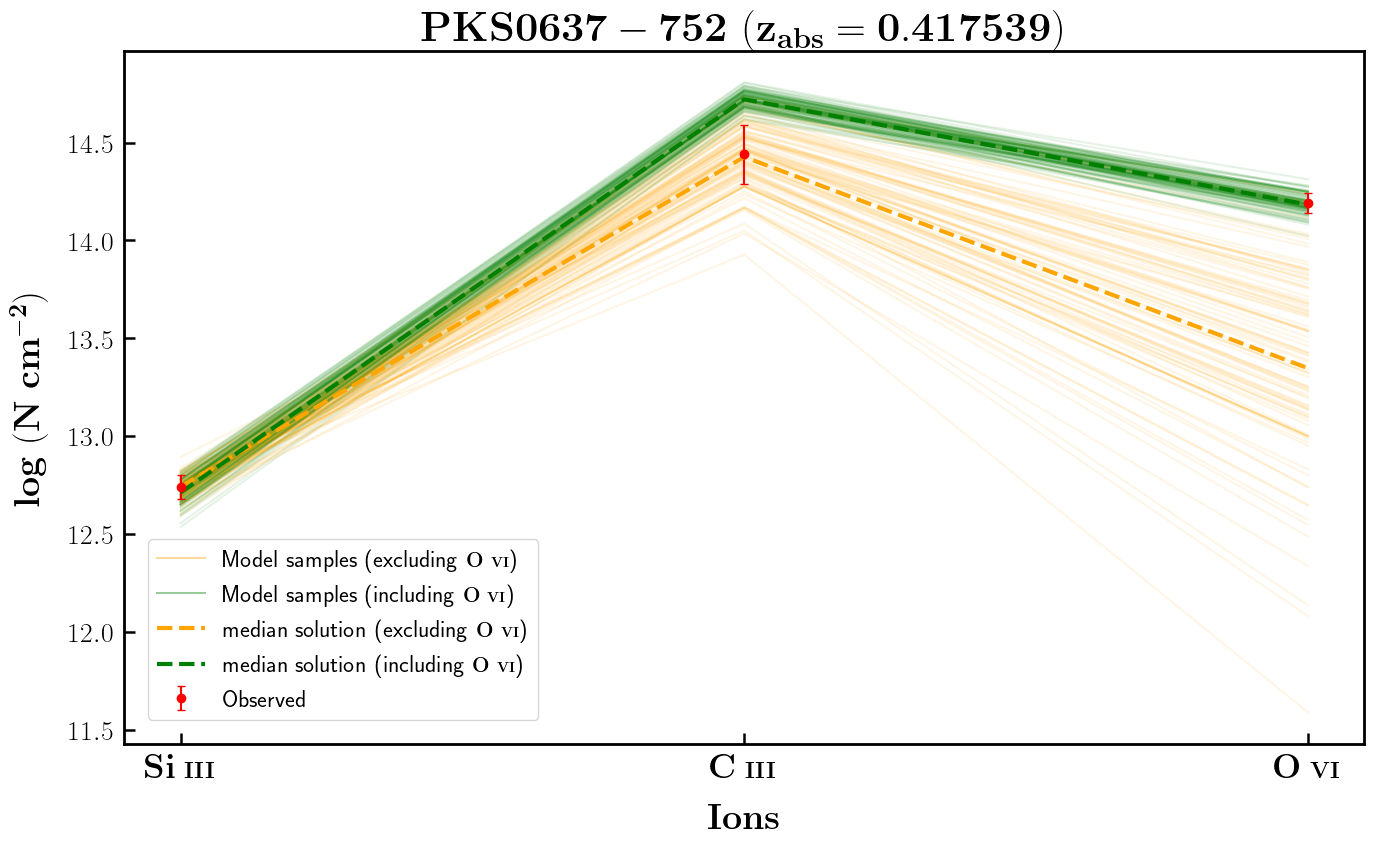
\includegraphics[width=1\linewidth]{Ionisation-Modelling-Plots/pks0637-z=0.417539-compI.png}




\newpage


\begin{landscape}

    \begin{figure}
    \centering
    \vspace{-20mm}
    \hspace*{-35mm}
    \captionsetup{oneside,margin={0cm,35mm}}
    \includegraphics[width=1.25\linewidth]{System-Plots/PG1424+240_z=0.147104_sys_plot.png}
    \end{figure}
    
\end{landscape}


\begin{center}
    
    \begin{tabular}{cccc}
            \hline \hline \tabularnewline
            \head{Ion} & \head{v (km s\textsuperscript{$\mathbf{-1}$})} & \head{b (km s\textsuperscript{$\mathbf{-1}$})} & \head{log [N cm\textsuperscript{$\mathbf{-2}$}]} 
            \tabularnewline \tabularnewline \hline \tabularnewline 
    
            \ion{C}{iv}   &    -81 $\pm$ 2    &    11 $\pm$ 4    &     13.58 $\pm$ 0.09 \\
            \ion{C}{iv}   &    -18 $\pm$ 2    &    20 $\pm$ 3    &     14.06 $\pm$ 0.05 \\ \tabularnewline
            \ion{Si}{iii}   &    -78 $\pm$ 2    &    15 $\pm$ 3    &     12.58 $\pm$ 0.05 \\
            \ion{Si}{iii}   &    -9 $\pm$ 1    &    16 $\pm$ 2    &     12.87 $\pm$ 0.03 \\ \tabularnewline
            \ion{Si}{iv}   &    -82 $\pm$ 4    &    13 $\pm$ 7    &     12.69 $\pm$ 0.1 \\
            \ion{Si}{iv}   &    -11 $\pm$ 2    &    11 $\pm$ 5    &     12.88 $\pm$ 0.07 \\ \tabularnewline
            \ion{O}{vi}   &    -56 $\pm$ 9    &    39 $\pm$ 13    &     13.77 $\pm$ 0.11 \\
            \ion{O}{vi}   &    4 $\pm$ 4    &    16 $\pm$ 6    &     13.73 $\pm$ 0.11 \\ \tabularnewline
            \ion{H}{i}   &    -454 $\pm$ 3    &    27 $\pm$ 5    &     13.16 $\pm$ 0.05 \\
            \ion{H}{i}   &    -87 $\pm$ 3    &    23 $\pm$ 2    &     14.88 $\pm$ 0.05 \\
            \ion{H}{i}   &    0 $\pm$ 3    &    29 $\pm$ 2    &     15.44 $\pm$ 0.14 \\
            \ion{H}{i}   &    216 $\pm$ 2    &    40 $\pm$ 3    &     13.49 $\pm$ 0.02 \\
            \tabularnewline \hline \hline \tabularnewline
    
    \end{tabular}
    
    \end{center}
    
    N(\ion{H}{I})=15.44 \\
    
    Excluding \ion{O}{vi} : $n_H$ = -3.81 $\pm$ 0.03 \hspace{10mm} $Z$ = -0.46 $\pm$ 0.03
    
    Including \ion{O}{vi} : $n_H$ = -3.88 $\pm$ 0.02 \hspace{10mm} $Z$ = -0.42 $\pm$ 0.02
    \\\\

    N(\ion{H}{I})=14.88 \\
    
    Excluding \ion{O}{vi} : $n_H$ = -3.74 $\pm$ 0.05 \hspace{10mm} $Z$ = -0.22 $\pm$ 0.04
    
    Including \ion{O}{vi} : $n_H$ = -3.96 $\pm$ 0.03 \hspace{10mm} $Z$ = -0.07 $\pm$ 0.04
    \\\\

    \newpage

    \begin{figure}[!h]
        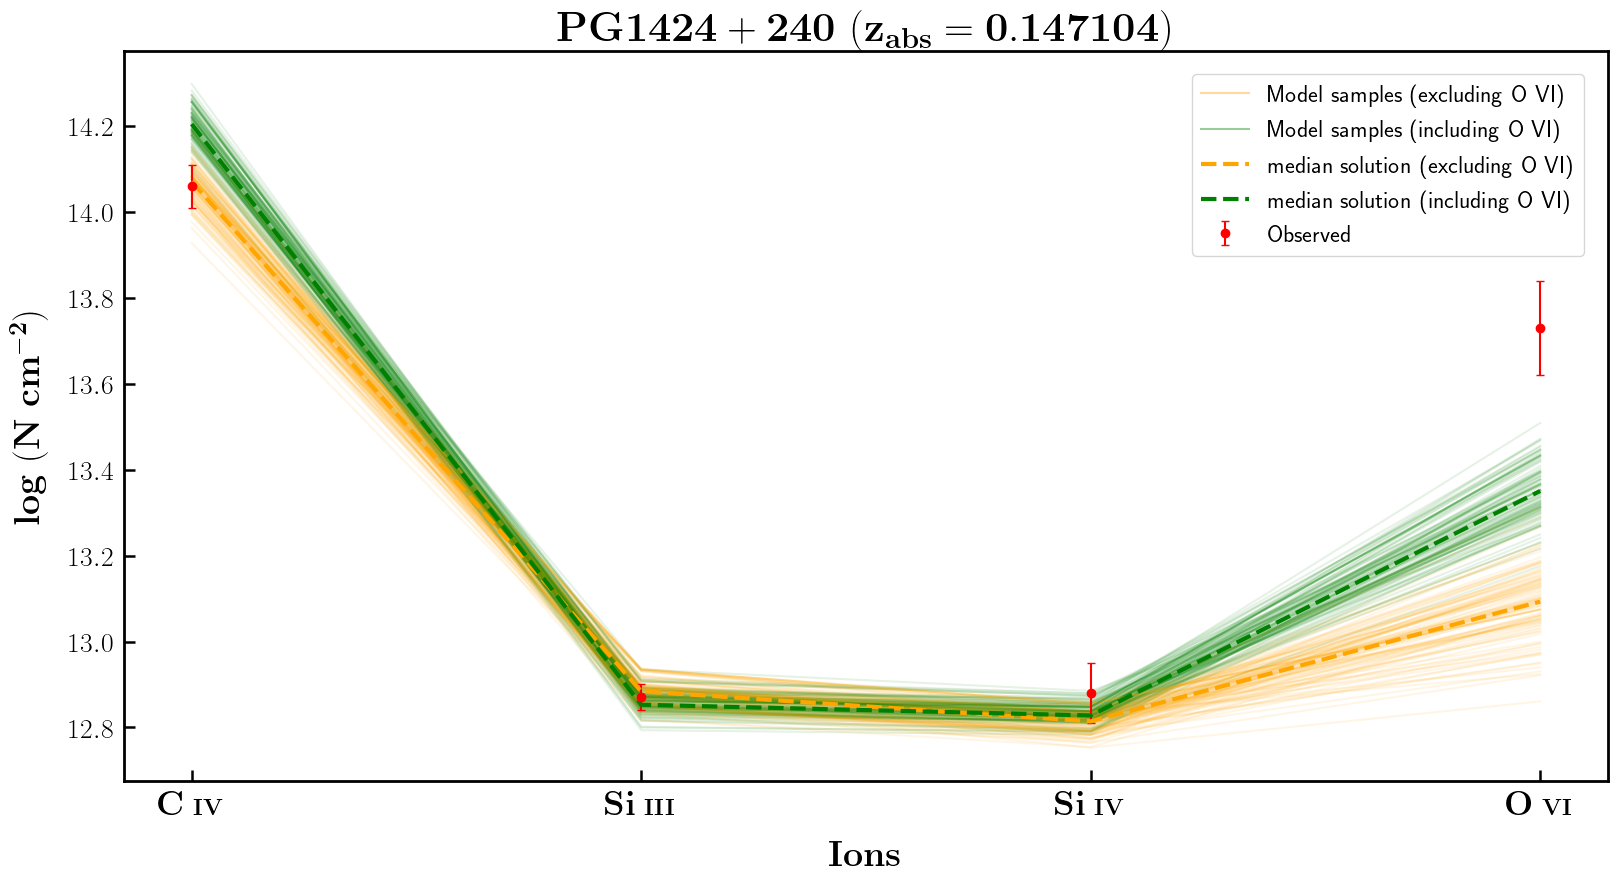
\includegraphics[width=0.9\linewidth]{Ionisation-Modelling-Plots/pg1424-z=0.147104-compIII.png}
        \caption{N(\ion{H}{i})=15.44}
    \end{figure}

    \begin{figure}[!b]
        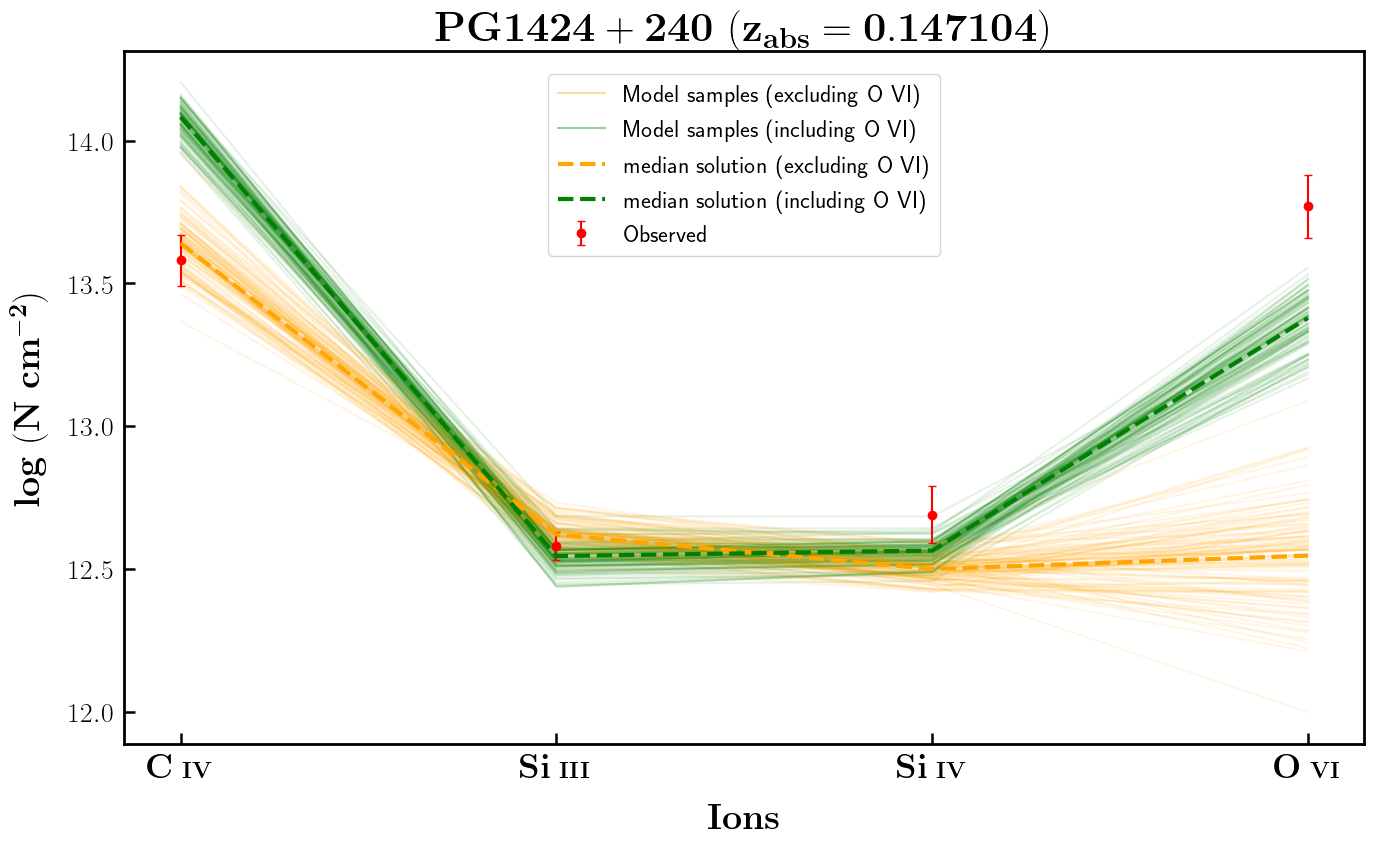
\includegraphics[width=0.9\linewidth]{Ionisation-Modelling-Plots/pg1424-z=0.147104-compII.png}
        \caption{N(\ion{H}{i})=14.88}
    \end{figure}

\newpage


\begin{landscape}

    \begin{figure}
    \centering
    \vspace{-20mm}
    \hspace*{-35mm}
    \captionsetup{oneside,margin={0cm,35mm}}
    \includegraphics[width=1.25\linewidth]{System-Plots/PG0003+158_z=0.386089_sys_plot.png}
    \end{figure}
    
\end{landscape}


\begin{center}
    
    \begin{tabular}{cccc}
        \hline \hline \tabularnewline
        \head{Ion} & \head{v (km s\textsuperscript{$\mathbf{-1}$})} & \head{b (km s\textsuperscript{$\mathbf{-1}$})} & \head{log [N cm\textsuperscript{$\mathbf{-2}$}]} 
        \tabularnewline \tabularnewline \hline \tabularnewline 
    
        \ion{O}{iii}   &    -18 $\pm$ 2    &    9 $\pm$ 5    &     13.93 $\pm$ 0.08 \\
        \ion{C}{iii}   &    -11 $\pm$ 1    &    13 $\pm$ 2    &     13.35 $\pm$ 0.05 \\
        \ion{N}{v}   &    -7 $\pm$ 1    &    33 $\pm$ 11    &     13.49 $\pm$ 0.11 \\
        \ion{O}{vi}   &    0 $\pm$ 2    &    25 $\pm$ 3    &     13.87 $\pm$ 0.04 \\
        \ion{O}{vi}   &    54 $\pm$ 3    &    25 $\pm$ 4    &     13.71 $\pm$ 0.06 \\
        \ion{H}{i}   &    -10 $\pm$ 1    &    29 $\pm$ 0    &     14.81 $\pm$ 0.03 \\
        \ion{H}{i}   &    40 $\pm$ 9    &    40 $\pm$ 4    &     14.1 $\pm$ 0.05 \\

        \tabularnewline \hline \hline \tabularnewline
    
    \end{tabular}
    
\end{center}
    
N(\ion{H}{I})=14.81 \\

Excluding \ion{O}{vi} : $n_H$ = -4.12 $\pm$ 0.06 \hspace{10mm} $Z$ = -0.65 $\pm$ 0.04

Including \ion{O}{vi} : $n_H$ = -4.07 $\pm$ 0.02 \hspace{10mm} $Z$ = -0.68 $\pm$ 0.03
\\\\
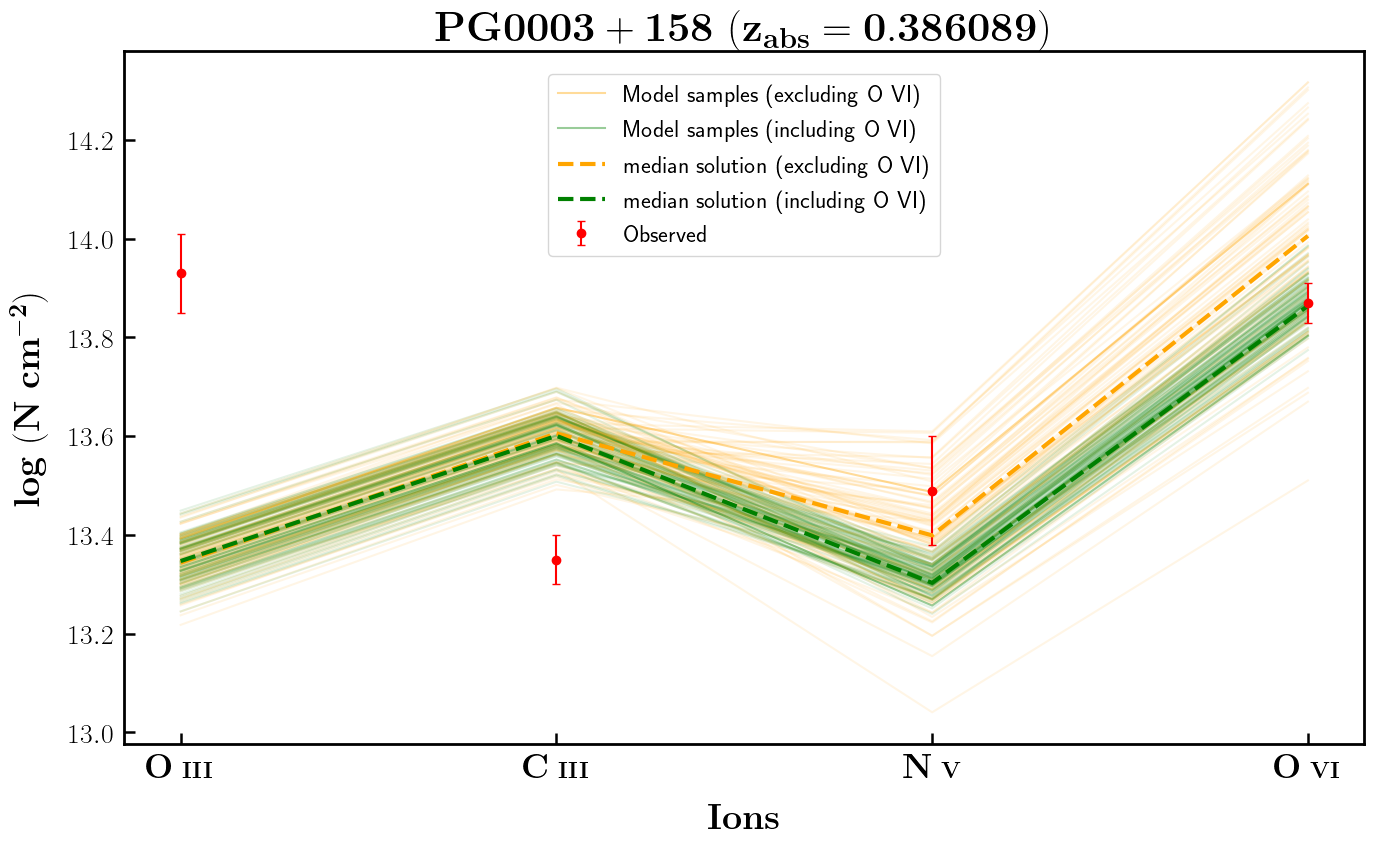
\includegraphics[width=1\linewidth]{Ionisation-Modelling-Plots/pg0003-z=0.386089-compI.png}



\newpage


\begin{landscape}

    \begin{figure}
    \centering
    \vspace{-20mm}
    \hspace*{-35mm}
    \captionsetup{oneside,margin={0cm,35mm}}
    \includegraphics[width=1.25\linewidth]{System-Plots/PG0003+158_z=0.421923_sys_plot.png}
    \end{figure}
    
\end{landscape}


\begin{center}
    
    \begin{tabular}{cccc}
        \hline \hline \tabularnewline
        \head{Ion} & \head{v (km s\textsuperscript{$\mathbf{-1}$})} & \head{b (km s\textsuperscript{$\mathbf{-1}$})} & \head{log [N cm\textsuperscript{$\mathbf{-2}$}]} 
        \tabularnewline \tabularnewline \hline \tabularnewline 
    
        \ion{C}{iii}   &    -9 $\pm$ 1    &    13 $\pm$ 1    &     13.35 $\pm$ 0.04 \\
        \ion{O}{iii}   &    -1 $\pm$ 2    &    7 $\pm$ 5    &     13.83 $\pm$ 0.13 \\
        \ion{O}{vi}   &    0 $\pm$ 1    &    27 $\pm$ 1    &     14.27 $\pm$ 0.02 \\
        \ion{H}{i}   &    -272 $\pm$ 6    &    66 $\pm$ 10    &     13.37 $\pm$ 0.05 \\
        \ion{H}{i}   &    -16 $\pm$ 1    &    64 $\pm$ 3    &     14.17 $\pm$ 0.04 \\
        \ion{H}{i}   &    -2 $\pm$ 1    &    26 $\pm$ 1    &     14.71 $\pm$ 0.02 \\
    
        \tabularnewline \hline \hline \tabularnewline
    
    \end{tabular}
    
\end{center}
    
N(\ion{H}{I})=14.17 \\

Excluding \ion{O}{vi} : $n_H$ = -2.66 $\pm$ 0.22 \hspace{10mm} $Z$ = 0.42 $\pm$ 0.23

Including \ion{O}{vi} : $n_H$ = -4.24 $\pm$ 0.02 \hspace{10mm} $Z$ = -0.09 $\pm$ 0.03 \\

NOTE : Convergence is not good for excluding \ion{O}{vi} case
\\\\
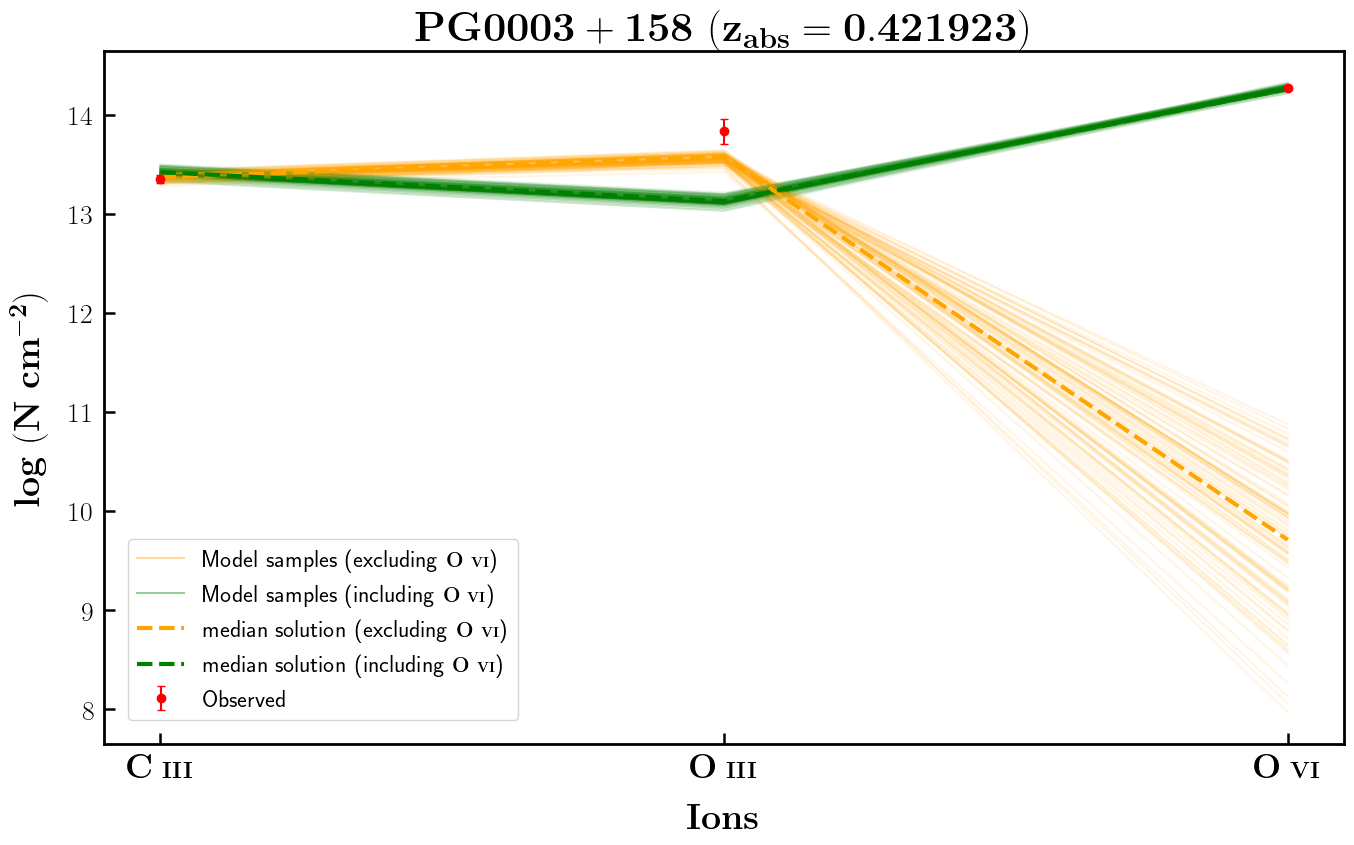
\includegraphics[width=1\linewidth]{Ionisation-Modelling-Plots/pg0003-z=0.421923-compII.png}
    


\newpage


\begin{landscape}

    \begin{figure}
    \centering
    \vspace{-20mm}
    \hspace*{-35mm}
    \captionsetup{oneside,margin={0cm,35mm}}
    \includegraphics[width=1.25\linewidth]{System-Plots/PG1216+069_z=0.282286_sys_plot.png}
    \end{figure}
    
\end{landscape}


\begin{center}
 
\begin{tabular}{cccc}
        \hline \hline \tabularnewline
        \head{Ion} & \head{v (km s\textsuperscript{$\mathbf{-1}$})} & \head{b (km s\textsuperscript{$\mathbf{-1}$})} & \head{log [N cm\textsuperscript{$\mathbf{-2}$}]} 
        \tabularnewline \tabularnewline \hline \tabularnewline 

        \ion{Si}{iii}   &    0 $\pm$ 1    &    14 $\pm$ 3    &     12.92 $\pm$ 0.05 \\
        \ion{C}{iii}   &    -51 $\pm$ 3    &    32 $\pm$ 5    &     13.33 $\pm$ 0.05 \\
        \ion{C}{iii}   &    5 $\pm$ 1    &    16 $\pm$ 2    &     13.76 $\pm$ 0.07 \\
        \ion{O}{vi}   &    -64 $\pm$ 6    &    58 $\pm$ 9    &     13.93 $\pm$ 0.05 \\
        \ion{O}{vi}   &    19 $\pm$ 2    &    12 $\pm$ 5    &     13.54 $\pm$ 0.09 \\
        \ion{H}{i}   &    -31 $\pm$ 1    &    52 $\pm$ 3    &     15.1 $\pm$ 0.05 \\
        \ion{H}{i}   &    7 $\pm$ 1    &    22 $\pm$ 1    &     16.4 $\pm$ 0.03 \\
        \ion{H}{i}   &    169 $\pm$ 22    &    53 $\pm$ 10    &     13.15 $\pm$ 0.18 \\

        \tabularnewline \hline \hline \tabularnewline

\end{tabular}
    
\end{center}
    
N(\ion{H}{I})=15.10 \\

Excluding \ion{O}{vi} : $n_H$ = -2.13 $\pm$ 0.15 \hspace{10mm} $Z$ = 0.65 $\pm$ 0.22

Including \ion{O}{vi} : $n_H$ = -3.86 $\pm$ 0.02 \hspace{10mm} $Z$ = -0.37 $\pm$ 0.03 \\

NOTE : Convergence is not much good for excluding \ion{O}{vi} case
\\\\

N(\ion{H}{I})=16.40 \\

Excluding \ion{O}{vi} : $n_H$ = -2.08 $\pm$ 0.43 \hspace{10mm} $Z$ = -0.37 $\pm$ 0.59

Including \ion{O}{vi} : $n_H$ = -3.68 $\pm$ 0.02 \hspace{10mm} $Z$ = -1.55 $\pm$ 0.04 \\

NOTE : Convergence is not much good for excluding \ion{O}{vi} case


\newpage


\begin{figure}[!h]
    \centering
    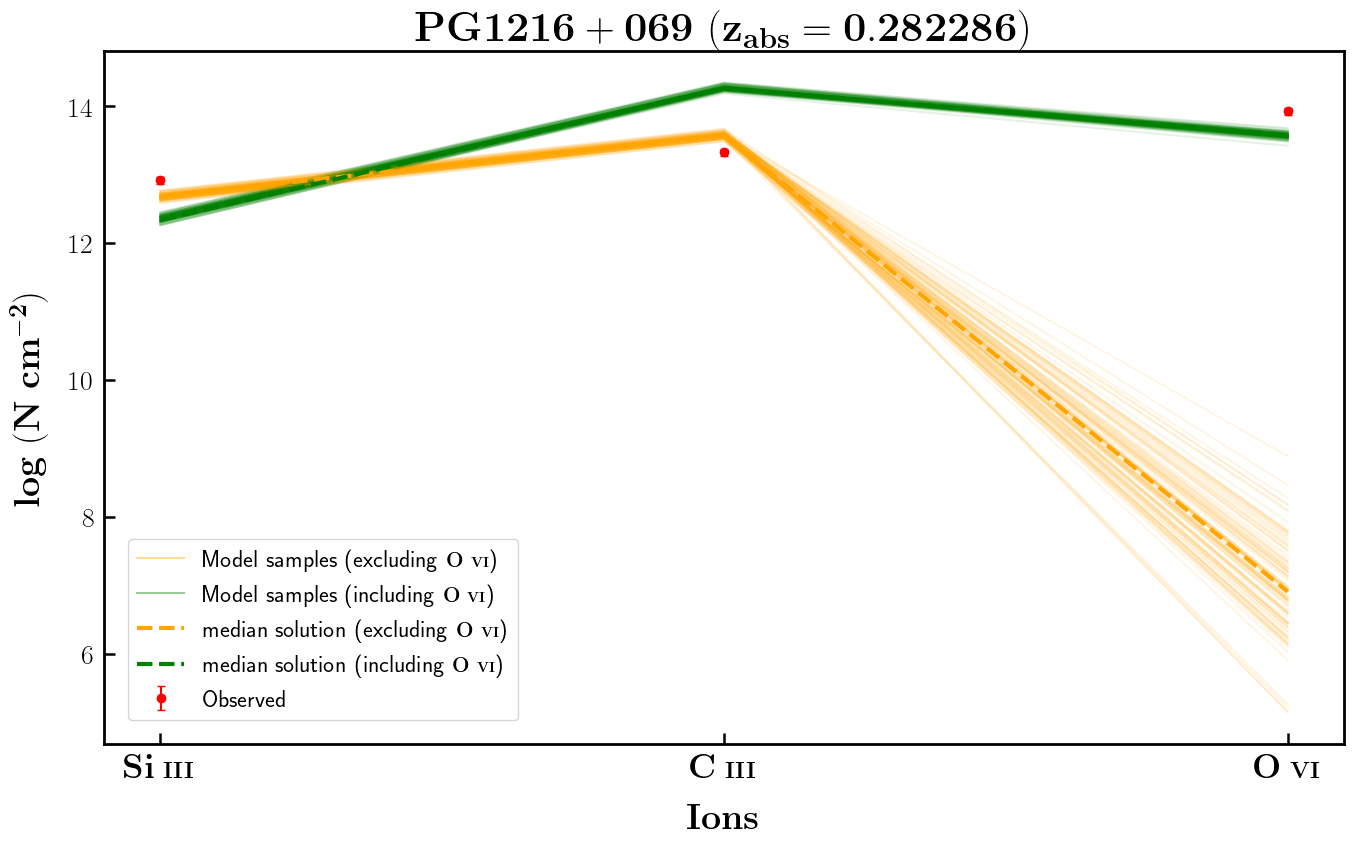
\includegraphics[width=0.85\linewidth]{Ionisation-Modelling-Plots/pg1216-z=0.282286-compI.png}
    \caption{N(\ion{H}{i})=15.10}
\end{figure}

\begin{figure}[!b]
    \centering
    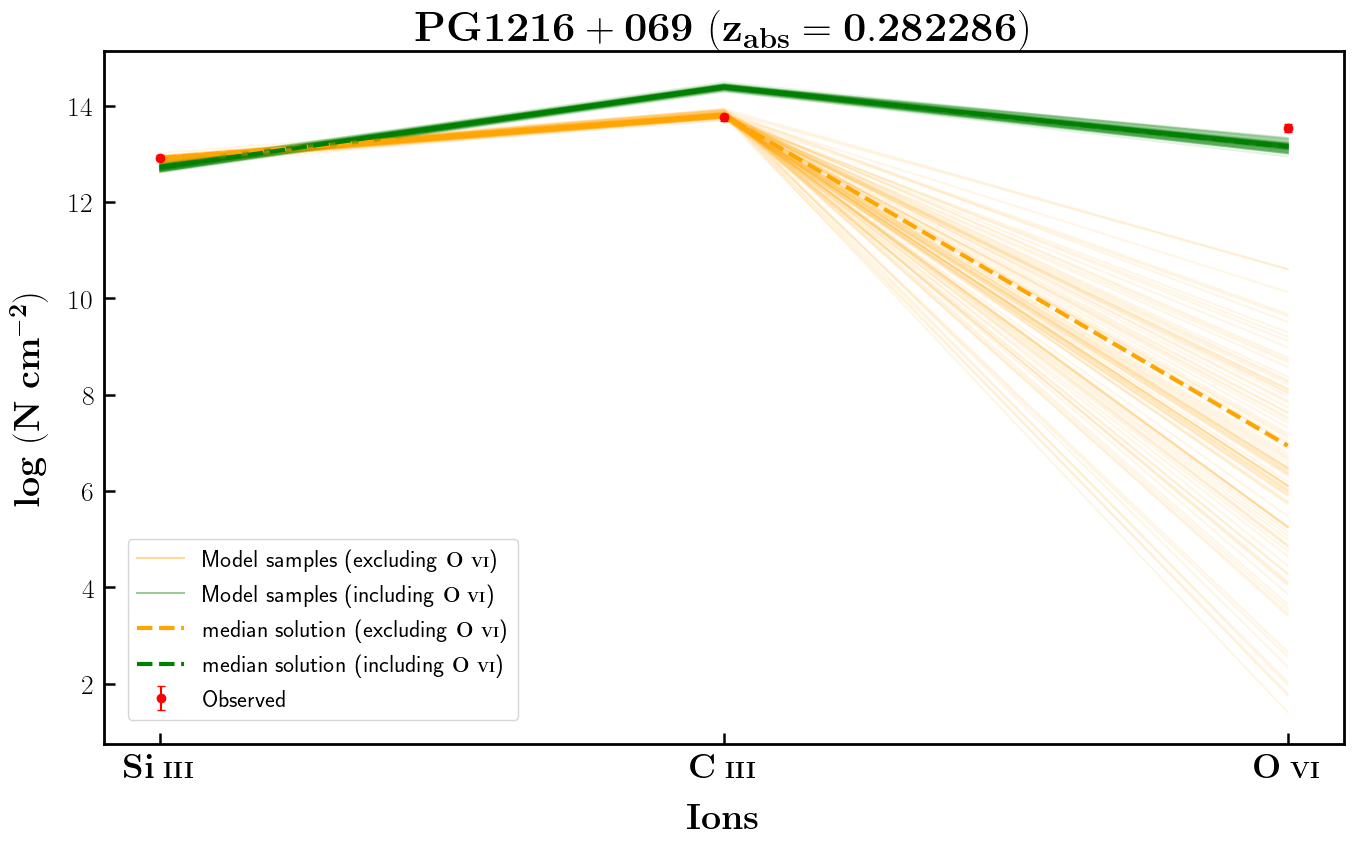
\includegraphics[width=0.85\linewidth]{Ionisation-Modelling-Plots/pg1216-z=0.282286-compII.png}
    \caption{N(\ion{H}{i})=16.40}
\end{figure}


\newpage

\begin{landscape}

\begin{figure}
    \centering
    \vspace{-20mm}
    \hspace*{-35mm}
    \captionsetup{oneside,margin={0cm,35mm}}
    \includegraphics[width=1.25\linewidth]{System-Plots/SDSSJ135712.61+170444_z=0.097869_sys_plot.png}
\end{figure}

\end{landscape}


\begin{center} 

\begin{tabular}{cccc} 

    \hline \hline \tabularnewline 
    \head{Ion} & \head{v (km s\textsuperscript{$\mathbf{-1}$})} & \head{b (km s\textsuperscript{$\mathbf{-1}$})} & \head{log [N cm\textsuperscript{$\mathbf{-2}$}]}
    \tabularnewline \tabularnewline \hline \tabularnewline 
 
    \ion{Si}{iii}   &    -62 $\pm$ 2    &    17 $\pm$ 3    &     12.94 $\pm$ 0.05 \\
    \ion{Si}{iii}   &    4 $\pm$ 1    &    13 $\pm$ 10    &     14.67 $\pm$ 2.87 \\
    \ion{C}{iv}   &    -74 $\pm$ 6    &    33 $\pm$ 1    &     13.82 $\pm$ 0.09 \\
    \ion{C}{iv}   &    -7 $\pm$ 8    &    32 $\pm$ 12    &     13.63 $\pm$ 0.12 \\
    \ion{Si}{iv}   &    -66 $\pm$ 4    &    18 $\pm$ 6    &     13.02 $\pm$ 0.08 \\
    \ion{Si}{iv}   &    0 $\pm$ 4    &    29 $\pm$ 5    &     13.3 $\pm$ 0.05 \\
    \ion{C}{ii}   &    -79 $\pm$ 8    &    19 $\pm$ 14    &     13.17 $\pm$ 0.16 \\
    \ion{C}{ii}   &    -1 $\pm$ 2    &    22 $\pm$ 3    &     13.92 $\pm$ 0.04 \\
    \ion{O}{vi}   &    -96 $\pm$ 10    &    43 $\pm$ 16    &     14.3 $\pm$ 0.11 \\
    \ion{H}{i}   &    -536 $\pm$ 3    &    29 $\pm$ 5    &     13.36 $\pm$ 0.05 \\
    \ion{H}{i}   &    -66 $\pm$ 0    &    29 $\pm$ 8    &     16.49 $\pm$ 0.12 \\
    \ion{H}{i}   &    0 $\pm$ 0    &    46 $\pm$ 4    &     15.01 $\pm$ 0.16 \\
    \ion{H}{i}   &    424 $\pm$ 3    &    34 $\pm$ 4    &     13.52 $\pm$ 0.04 \\

    \tabularnewline \hline \hline \tabularnewline 

\end{tabular}

\end{center}

N(\ion{H}{I})=16.49 \\

Excluding \ion{O}{vi} : $n_H$ = -3.76 $\pm$ 0.05 \hspace{10mm} $Z$ = -1.49 $\pm$ 0.04

Including \ion{O}{vi} : $n_H$ = -4.06 $\pm$ 0.02 \hspace{10mm} $Z$ = -1.32 $\pm$ 0.04
\\\\

N(\ion{H}{I})=15.01 \\

Excluding \ion{O}{vi} : $n_H$ = -3.25 $\pm$ 0.04 \hspace{10mm} $Z$ = 0.93 $\pm$ 0.04

Including \ion{O}{vi} : $n_H$ = -3.84 $\pm$ 0.03 \hspace{10mm} $Z$ = 0.75 $\pm$ 0.03
\\\\
NOTE : Using \ion{O}{vi} column density from other component to compare.

\newpage


\begin{figure}[!h]
    \centering
    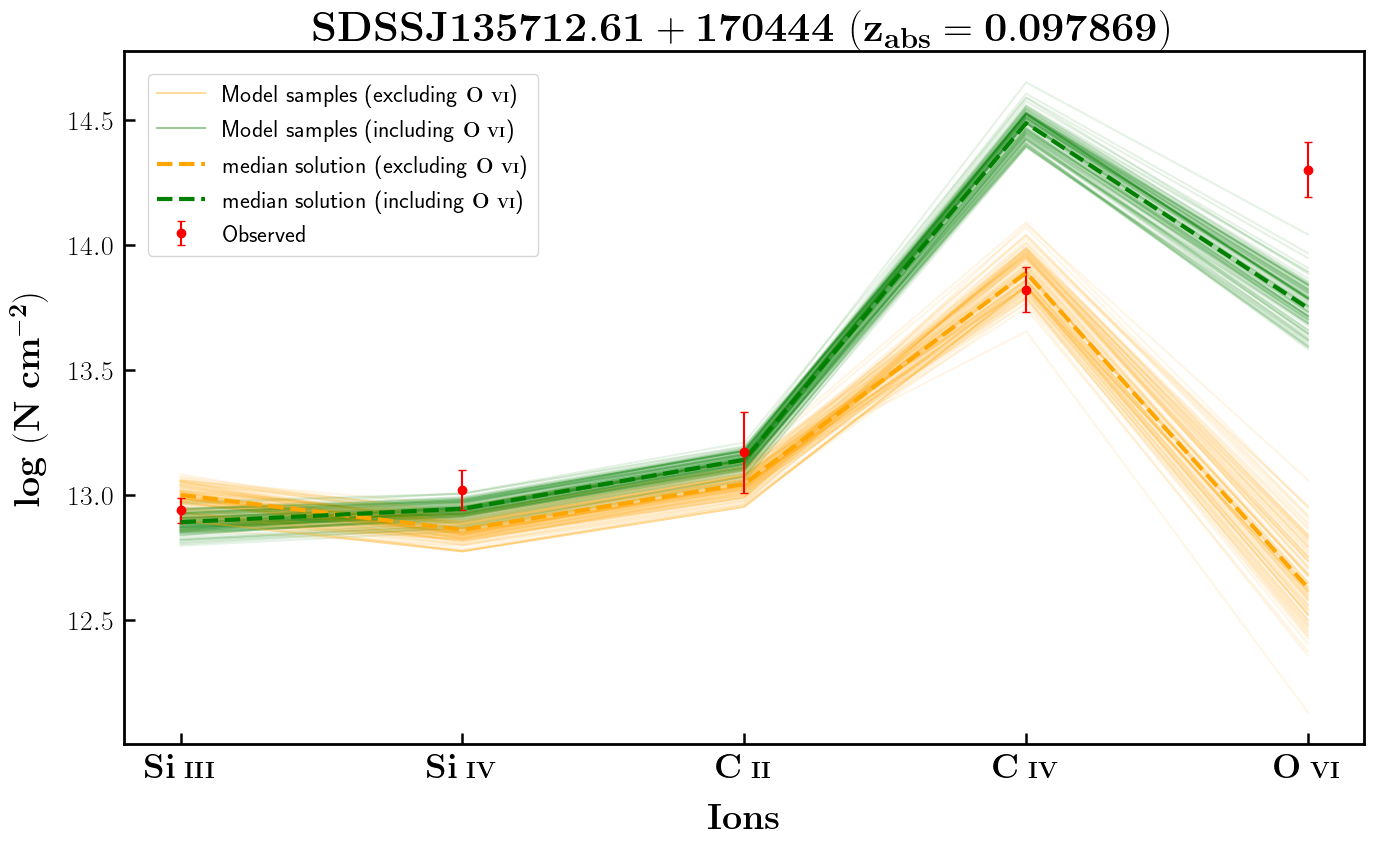
\includegraphics[width=0.85\linewidth]{Ionisation-Modelling-Plots/s135712-z=0.097869-compII.png}
    \caption{N(\ion{H}{i})=16.49}
\end{figure}

\begin{figure}[!b]
    \centering
    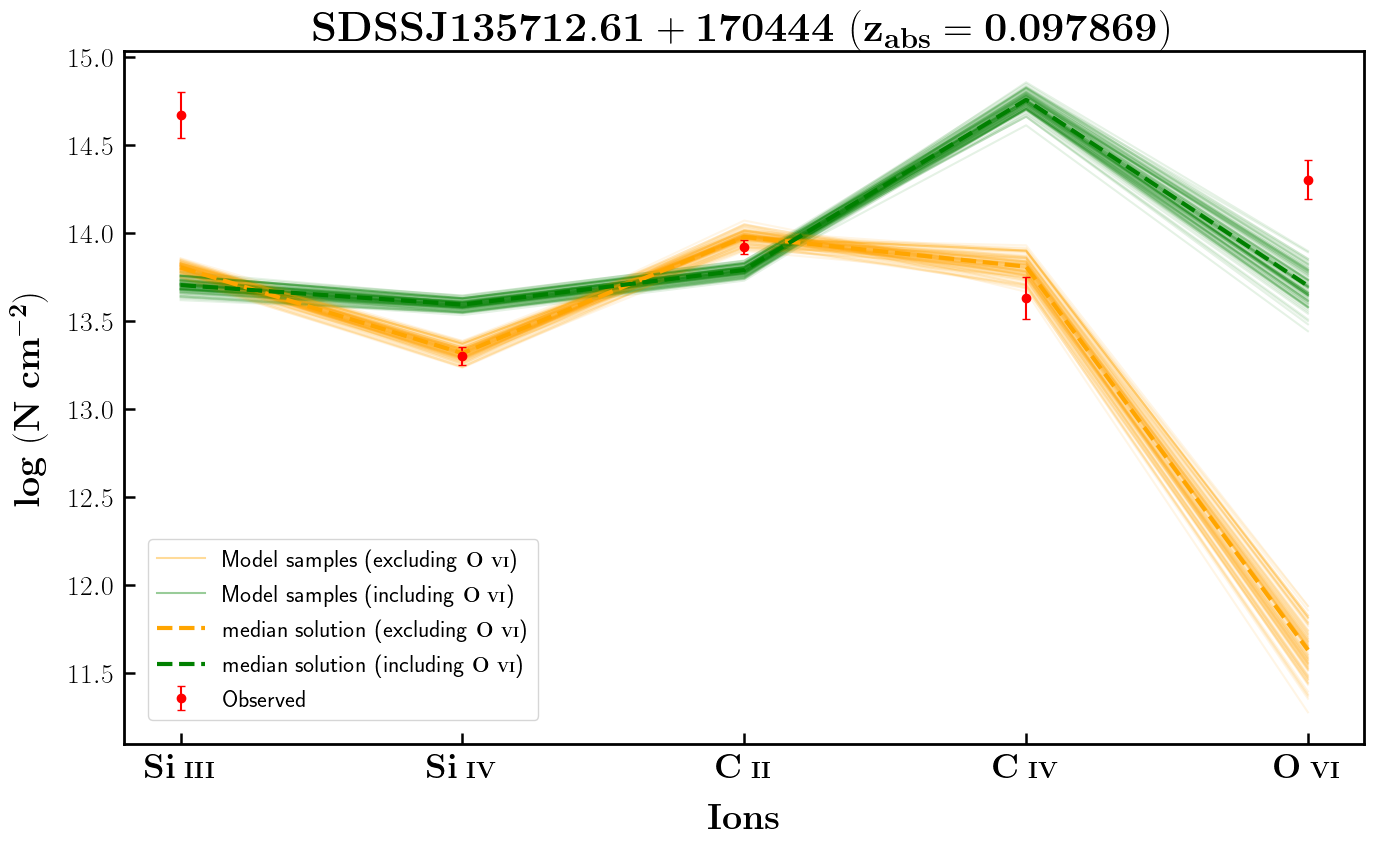
\includegraphics[width=0.85\linewidth]{Ionisation-Modelling-Plots/s135712-z=0.097869-compIII.png}
    \caption{N(\ion{H}{i})=15.01}
\end{figure}



\newpage

\begin{landscape}

\begin{figure}
    \centering
    \vspace{-20mm}
    \hspace*{-35mm}
    \captionsetup{oneside,margin={0cm,35mm}}
    \includegraphics[width=1.25\linewidth]{System-Plots/1ES1553+113_z=0.187764_sys_plot.png}
\end{figure}

\end{landscape}


\begin{center} 

\begin{tabular}{cccc} 

    \hline \hline \tabularnewline 
    \head{Ion} & \head{v (km s\textsuperscript{$\mathbf{-1}$})} & \head{b (km s\textsuperscript{$\mathbf{-1}$})} & \head{log [N cm\textsuperscript{$\mathbf{-2}$}]}
    \tabularnewline \tabularnewline \hline \tabularnewline 
 
    \ion{C}{iii}   &    -46 $\pm$ 1    &    5 $\pm$ 4    &     13.17 $\pm$ 0.46 \\
    \ion{C}{iii}   &    -6 $\pm$ 1    &    13 $\pm$ 2    &     13.21 $\pm$ 0.03 \\
    \ion{N}{v}   &    -47 $\pm$ 2    &    17 $\pm$ 0    &     13.43 $\pm$ 0.05 \\
    \ion{N}{v}   &    -5 $\pm$ 2    &    16 $\pm$ 4    &     13.33 $\pm$ 0.06 \\
    \ion{O}{vi}   &    -42 $\pm$ 1    &    3 $\pm$ 1    &     14.23 $\pm$ 0.33 \\
    \ion{O}{vi}   &    0 $\pm$ 1    &    15 $\pm$ 3    &     13.71 $\pm$ 0.03 \\
    \ion{O}{vi}   &    511 $\pm$ 3    &    28 $\pm$ 5    &     13.49 $\pm$ 0.05 \\
    \ion{H}{i}   &    -52 $\pm$ 3    &    8 $\pm$ 6    &     12.76 $\pm$ 0.15 \\
    \ion{H}{i}   &    -28 $\pm$ 1    &    51 $\pm$ 1    &     13.88 $\pm$ 0.01 \\
    \ion{H}{i}   &    425 $\pm$ 3    &    25 $\pm$ 5    &     13.02 $\pm$ 0.07 \\
    \ion{H}{i}   &    496 $\pm$ 2    &    37 $\pm$ 3    &     13.46 $\pm$ 0.03 \\

    \tabularnewline \hline \hline \tabularnewline 

\end{tabular}

\end{center}

N(\ion{H}{I})=12.76 \\

Excluding \ion{O}{vi} : $n_H$ = -4.62 $\pm$ 0.04 \hspace{10mm} $Z$ = 1.37 $\pm$ 0.06

Including \ion{O}{vi} : $n_H$ = -4.63 $\pm$ 0.03 \hspace{10mm} $Z$ = 1.37 $\pm$ 0.06
\\\\
NOTE : Reference metallicity at log Z = 1. Low N(\ion{H}{I}), and error for column density for \ion{C}{iii} and \ion{O}{vi} for component I were obtained from $\chi^2$, else they were large and convergence was not good. Nearly similar solution for both the cases. \\

N(\ion{H}{I})=13.88 \\

Excluding \ion{O}{vi} : $n_H$ = -4.6 $\pm$ 0.04 \hspace{10mm} $Z$ = 0.03 $\pm$ 0.03

Including \ion{O}{vi} : $n_H$ = -4.44 $\pm$ 0.02 \hspace{10mm} $Z$ = -0.06 $\pm$ 0.02
\\\\


\newpage


\begin{figure}[!h]
    \centering
    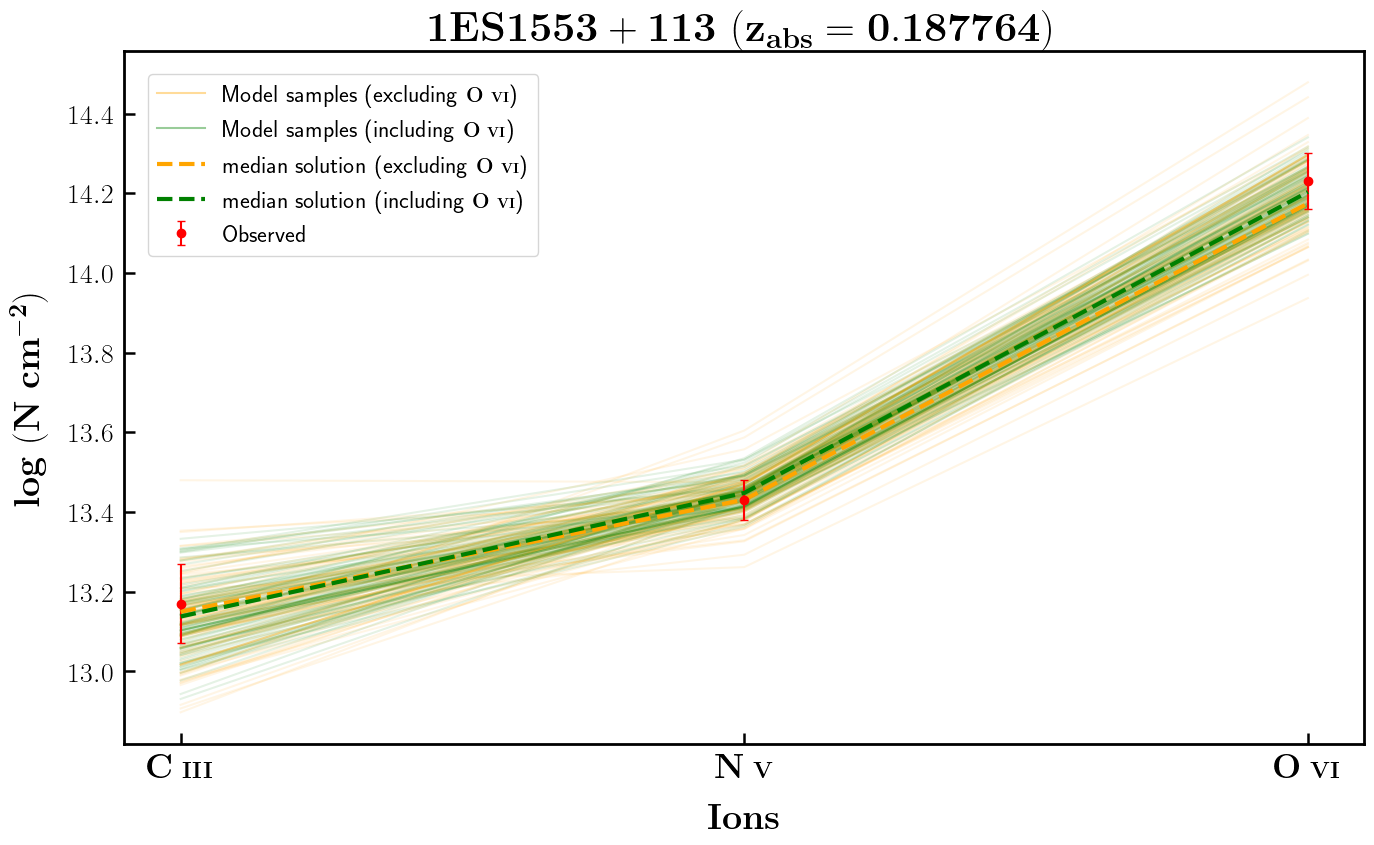
\includegraphics[width=0.85\linewidth]{Ionisation-Modelling-Plots/1es1553-z=0.187764-compI.png}
    \caption{N(\ion{H}{i})=12.76}
\end{figure}

\begin{figure}[!b]
    \centering
    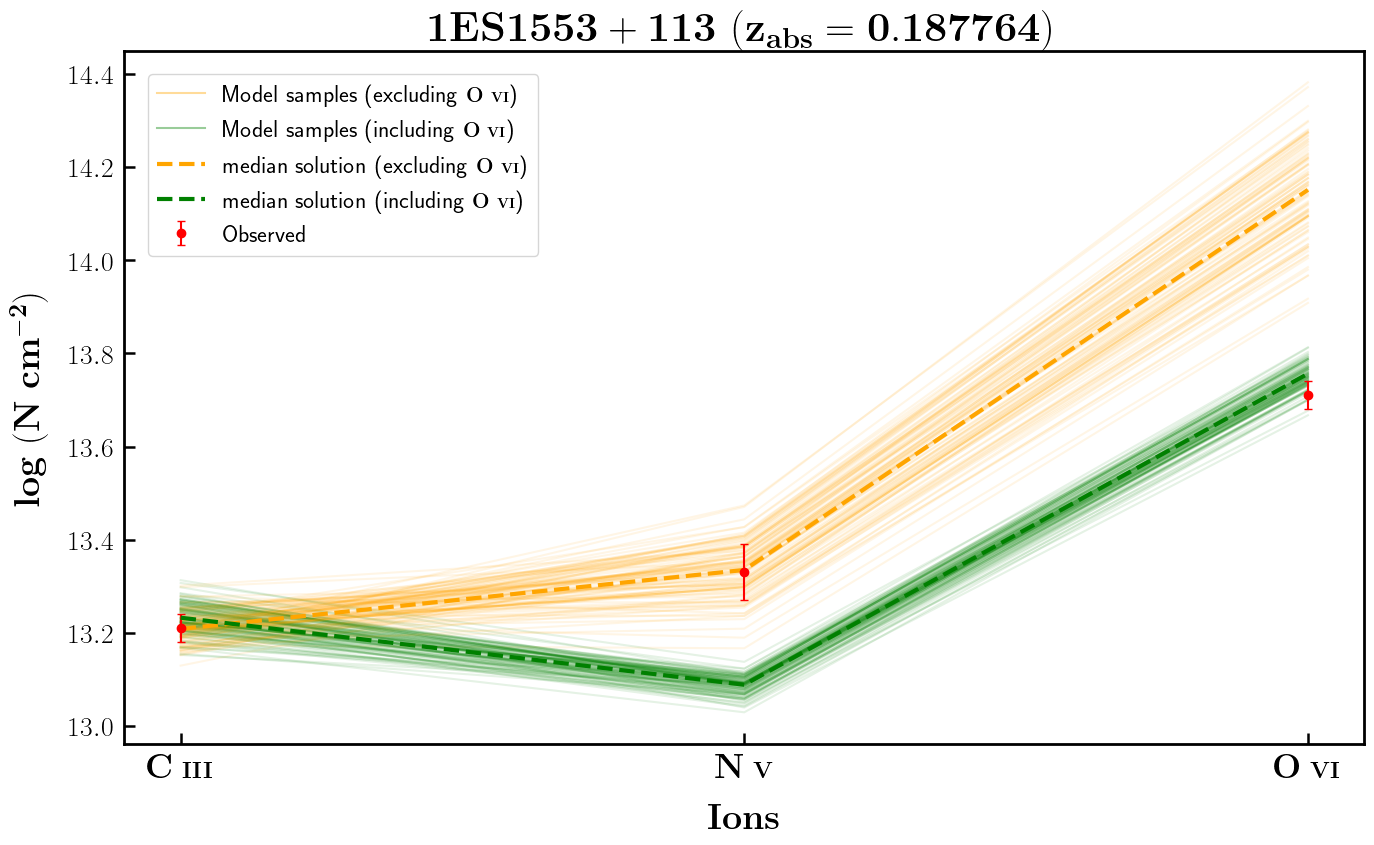
\includegraphics[width=0.85\linewidth]{Ionisation-Modelling-Plots/1es1553-z=0.187764-compII.png}
    \caption{N(\ion{H}{i})=13.88}
\end{figure}



\newpage

\begin{landscape}

\begin{figure}
    \centering
    \vspace{-20mm}
    \hspace*{-35mm}
    \captionsetup{oneside,margin={0cm,35mm}}
    \includegraphics[width=1.25\linewidth]{System-Plots/SBS1108+560_z=0.463207_sys_plot.png}
\end{figure}

\end{landscape}


\begin{center} 

\begin{tabular}{cccc} 

    \hline \hline \tabularnewline 
    \head{Ion} & \head{v (km s\textsuperscript{$\mathbf{-1}$})} & \head{b (km s\textsuperscript{$\mathbf{-1}$})} & \head{log [N cm\textsuperscript{$\mathbf{-2}$}]}
    \tabularnewline \tabularnewline \hline \tabularnewline 
 
    \ion{O}{i}   &    25 $\pm$ 2    &    18 $\pm$ 4    &     14.13 $\pm$ 0.05 \\
    \ion{Si}{iii}   &    -23 $\pm$ 9    &    39 $\pm$ 12    &     13.26 $\pm$ 0.12 \\
    \ion{Si}{iii}   &    21 $\pm$ 2    &    13 $\pm$ 15    &     14.61 $\pm$ 0.24 \\
    \ion{C}{ii}   &    12 $\pm$ 9    &    31 $\pm$ 4    &     14.15 $\pm$ 0.05 \\
    \ion{C}{ii}   &    34 $\pm$ 2    &    12 $\pm$ 5    &     14.67 $\pm$ 0.1 \\
    \ion{C}{iii}   &    -48 $\pm$ 3    &    15 $\pm$ 1    &     13.66 $\pm$ 0.08 \\
    \ion{C}{iii}   &    -10 $\pm$ 3    &    26 $\pm$ 7    &     14.16 $\pm$ 0.07 \\
    \ion{C}{iii}   &    28 $\pm$ 3    &    24 $\pm$ 1    &     13.95 $\pm$ 0.05 \\
    \ion{N}{iii}   &    -22 $\pm$ 59    &    67 $\pm$ 61    &     13.77 $\pm$ 0.1 \\
    \ion{N}{iii}   &    32 $\pm$ 2    &    26 $\pm$ 4    &     14.49 $\pm$ 0.09 \\
    \ion{Si}{ii}   &    25 $\pm$ 1    &    15 $\pm$ 1    &     13.57 $\pm$ 0.08 \\
    \ion{O}{vi}   &    0 $\pm$ 6    &    45 $\pm$ 10    &     13.71 $\pm$ 0.07 \\
    \ion{H}{i}   &    -48 $\pm$ 0    &    22 $\pm$ 2    &     15.77 $\pm$ 0.02 \\
    \ion{H}{i}   &    -10 $\pm$ 2    &    16 $\pm$ 0    &     15.79 $\pm$ 0.11 \\
    \ion{H}{i}   &    28 $\pm$ 1    &    16 $\pm$ 1    &     18.1 $\pm$ 0.12 \\
    
    \tabularnewline \hline \hline \tabularnewline 

\end{tabular}

\end{center}

N(\ion{H}{I})=18.10 \\

Excluding \ion{O}{vi} : $n_H$ = -1.88 $\pm$ 0.03 \hspace{10mm} $Z$ = 1.07 $\pm$ 0.04

Including \ion{O}{vi} : $n_H$ = -2.83 $\pm$ 0.02 \hspace{10mm} $Z$ = 0.89 $\pm$ 0.03
\\\\
NOTE : Using \ion{O}{vi} from other component to compare
\\\\
N(\ion{H}{I})=15.79 \\

Excluding \ion{O}{vi} : $n_H$ = -2.65 $\pm$ 0.22 \hspace{10mm} $Z$ = 1.6 $\pm$ 0.22

Including \ion{O}{vi} : $n_H$ = -3.56 $\pm$ 0.03 \hspace{10mm} $Z$ = 1.16 $\pm$ 0.05
\\\\
NOTE : log Z is around 1 in both the components.

\newpage

\begin{figure}[!h]
    \centering
    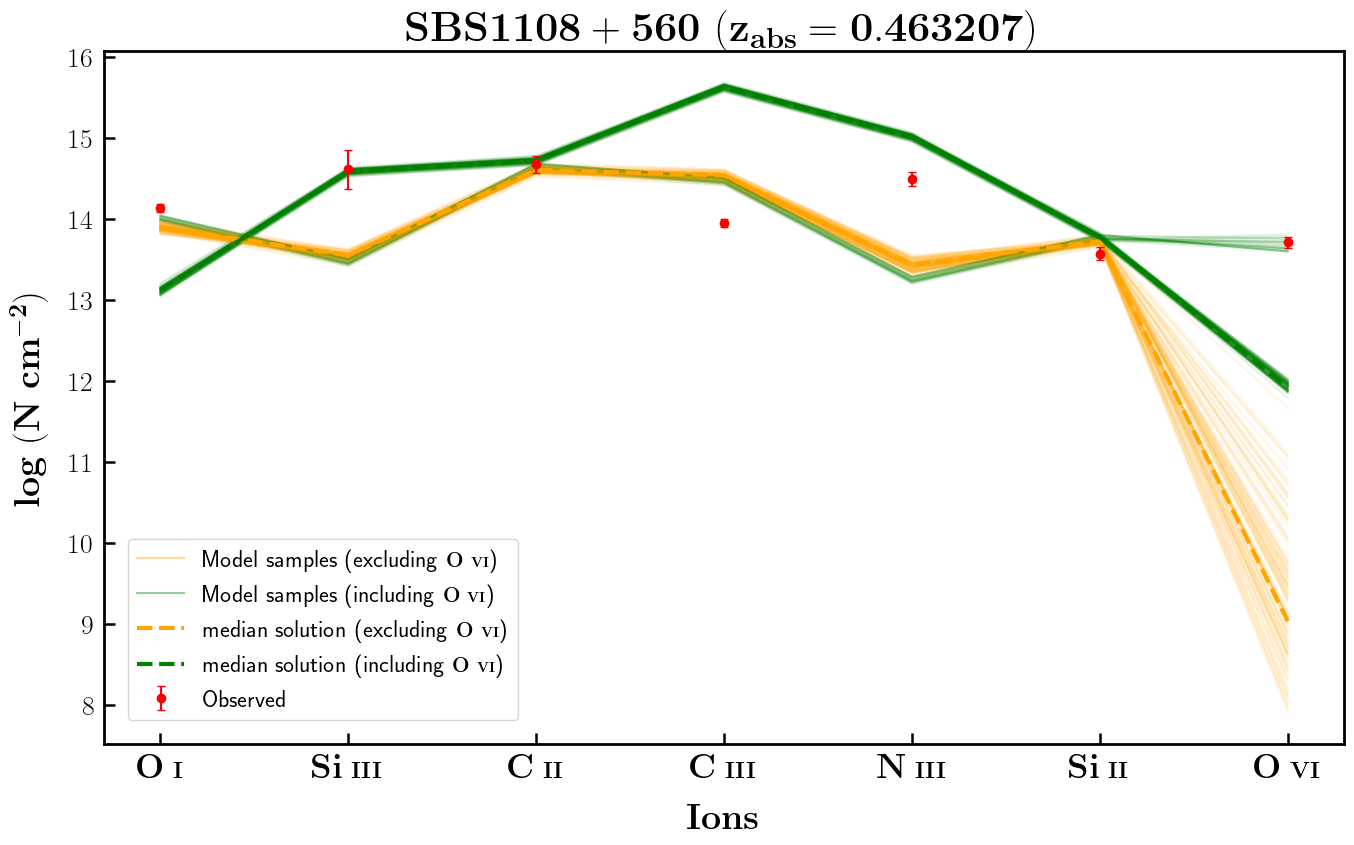
\includegraphics[width=0.85\linewidth]{Ionisation-Modelling-Plots/sbs1108-z=0.463207-compIII.png}
    \caption{N(\ion{H}{i})=18.10}
\end{figure}

\begin{figure}[!b]
    \centering
    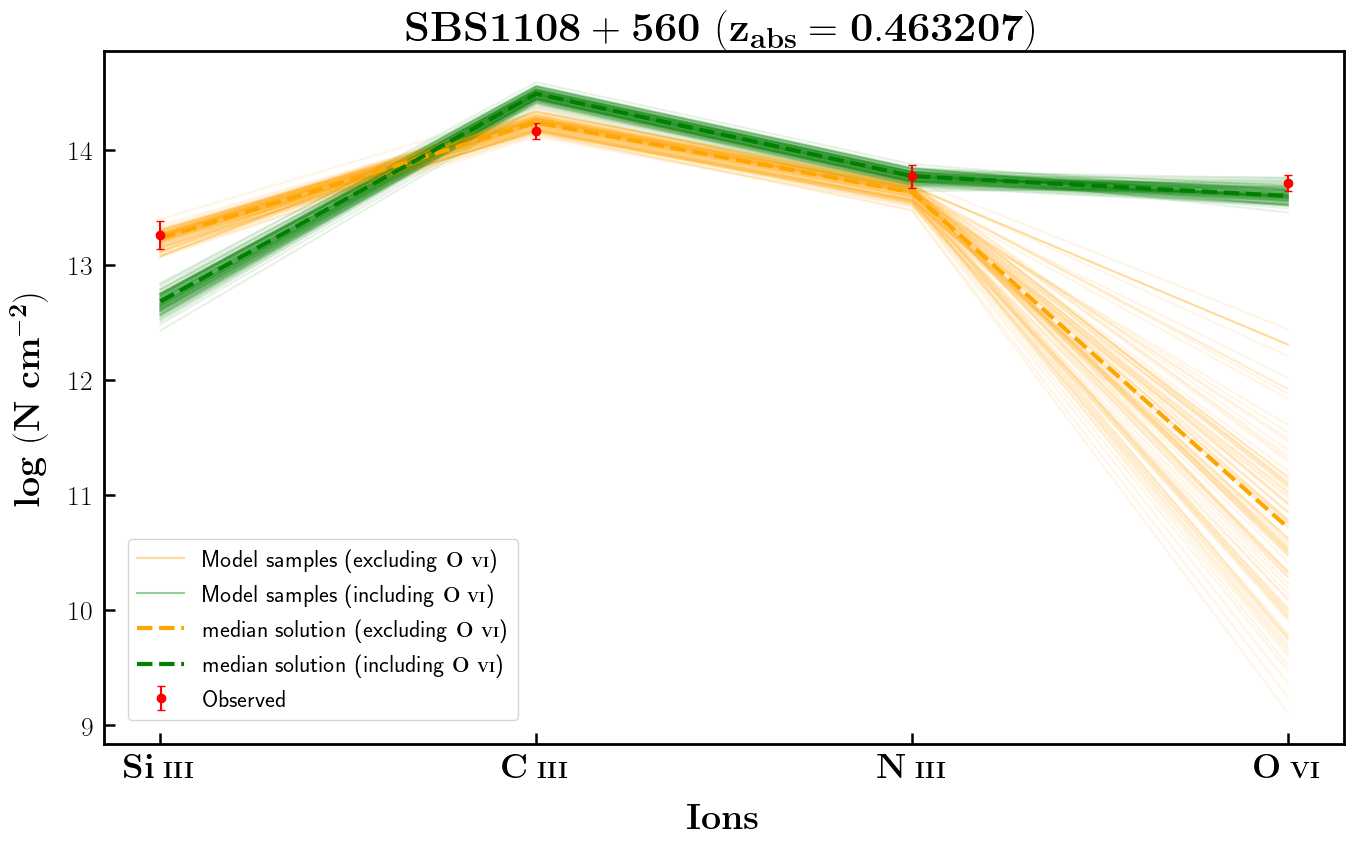
\includegraphics[width=0.85\linewidth]{Ionisation-Modelling-Plots/sbs1108-z=0.463207-compII.png}
    \caption{N(\ion{H}{i})=15.79}
\end{figure}



\newpage

\begin{landscape}

\begin{figure}
    \centering
    \vspace{-20mm}
    \hspace*{-35mm}
    \captionsetup{oneside,margin={0cm,35mm}}
    \includegraphics[width=1.25\linewidth]{System-Plots/PG1222+216_z=0.378389_sys_plot.png}
\end{figure}

\end{landscape}


\begin{center} 

\begin{tabular}{cccc} 

    \hline \hline \tabularnewline 
    \head{Ion} & \head{v (km s\textsuperscript{$\mathbf{-1}$})} & \head{b (km s\textsuperscript{$\mathbf{-1}$})} & \head{log [N cm\textsuperscript{$\mathbf{-2}$}]}
    \tabularnewline \tabularnewline \hline \tabularnewline 
 
    \ion{O}{iii}   &    7 $\pm$ 5    &    61 $\pm$ 8    &     14.51 $\pm$ 0.04 \\
    \ion{Si}{iii}   &    0 $\pm$ 2    &    30 $\pm$ 3    &     12.98 $\pm$ 0.03 \\
    \ion{C}{iii}   &    -261 $\pm$ 3    &    17 $\pm$ 5    &     13.54 $\pm$ 0.06 \\
    \ion{C}{iii}   &    -215 $\pm$ 5    &    22 $\pm$ 6    &     13.40 $\pm$ 0.08 \\
    \ion{C}{iii}   &    0 $\pm$ 2    &    32 $\pm$ 3    &     13.79 $\pm$ 0.02 \\
    \ion{C}{iii}   &    63 $\pm$ 3    &    13 $\pm$ 6    &     13.12 $\pm$ 0.07 \\
    \ion{O}{vi}   &    -439 $\pm$ 3    &    28 $\pm$ 5    &     13.42 $\pm$ 0.06 \\
    \ion{O}{vi}   &    -264 $\pm$ 6    &    24 $\pm$ 6    &     13.75 $\pm$ 0.2 \\
    \ion{O}{vi}   &    -223 $\pm$ 14    &    34 $\pm$ 13    &     13.68 $\pm$ 0.24 \\
    \ion{O}{vi}   &    -24 $\pm$ 12    &    14 $\pm$ 18    &     13.00 $\pm$ 0.11 \\
    \ion{O}{vi}   &    13 $\pm$ 4    &    29 $\pm$ 13    &     13.95 $\pm$ 0.16 \\
    \ion{O}{vi}   &    59 $\pm$ 6    &    18 $\pm$ 7    &     13.42 $\pm$ 0.23 \\
    \ion{H}{i}   &    -455 $\pm$ 3    &    26 $\pm$ 4    &     13.40 $\pm$ 0.06 \\
    \ion{H}{i}   &    -353 $\pm$ 9    &    64 $\pm$ 19    &     13.54 $\pm$ 0.11 \\
    \ion{H}{i}   &    -268 $\pm$ 1    &    16 $\pm$ 6    &     13.70 $\pm$ 0.14 \\
    \ion{H}{i}   &    -227 $\pm$ 5    &    52 $\pm$ 4    &     14.34 $\pm$ 0.05 \\
    \ion{H}{i}   &    -27 $\pm$ 2    &    23 $\pm$ 1    &     14.73 $\pm$ 0.08 \\
    \ion{H}{i}   &    31 $\pm$ 2    &    43 $\pm$ 1    &     15.43 $\pm$ 0.04 \\
    
    \tabularnewline \hline \hline \tabularnewline 

\end{tabular}

\end{center}

N(\ion{H}{I})=15.43 \\

Excluding \ion{O}{vi} : $n_H$ = -2.66 $\pm$ 0.05 \hspace{10mm} $Z$ = -0.25 $\pm$ 0.06

Including \ion{O}{vi} : $n_H$ = -3.16 $\pm$ 0.03 \hspace{10mm} $Z$ = -0.66 $\pm$ 0.02
\\\\
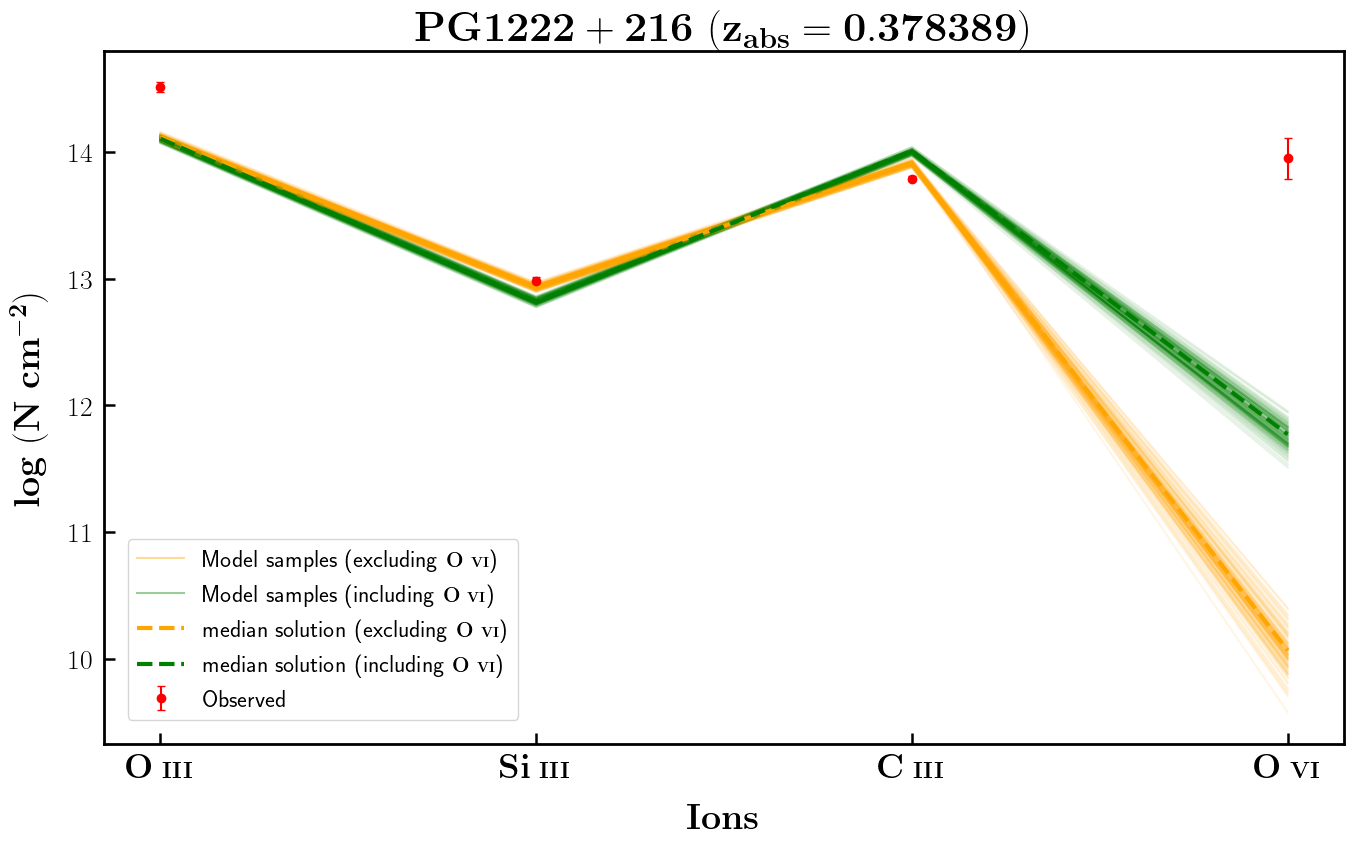
\includegraphics[width=1\linewidth]{Ionisation-Modelling-Plots/pg1222-z=0.378389-compVI.png}



\newpage

\begin{landscape}

\begin{figure}
    \centering
    \vspace{-20mm}
    \hspace*{-35mm}
    \captionsetup{oneside,margin={0cm,35mm}}
    \includegraphics[width=1.25\linewidth]{System-Plots/PG1116+215_z=0.138527_sys_plot.png}
\end{figure}

\end{landscape}


\begin{center} 

\begin{tabular}{cccc} 

    \hline \hline \tabularnewline 
    \head{Ion} & \head{v (km s\textsuperscript{$\mathbf{-1}$})} & \head{b (km s\textsuperscript{$\mathbf{-1}$})} & \head{log [N cm\textsuperscript{$\mathbf{-2}$}]}
    \tabularnewline \tabularnewline \hline \tabularnewline 
 
    \ion{N}{v}   &    -7 $\pm$ 3    &    12 $\pm$ 6    &     12.84 $\pm$ 0.09 \\
    \ion{N}{ii}   &    -5 $\pm$ 1    &    6 $\pm$ 3    &     13.62 $\pm$ 0.11 \\
    \ion{N}{ii}   &    33 $\pm$ 6    &    8 $\pm$ 13    &     12.85 $\pm$ 0.15 \\
    \ion{P}{ii}   &    -44 $\pm$ 5    &    19 $\pm$ 8    &     12.94 $\pm$ 0.09 \\
    \ion{Si}{ii}   &    -13 $\pm$ 1    &    9 $\pm$ 1    &     12.46 $\pm$ 0.06 \\
    \ion{Si}{ii}   &    13 $\pm$ 1    &    23 $\pm$ 3    &     12.31 $\pm$ 0.04 \\
    \ion{Si}{iii}   &    -9 $\pm$ 1    &    10 $\pm$ 1    &     12.92 $\pm$ 0.04 \\
    \ion{Si}{iv}   &    -13 $\pm$ 2    &    4 $\pm$ 3    &     12.84 $\pm$ 0.09 \\
    \ion{O}{vi}   &    -1 $\pm$ 1    &    35 $\pm$ 3    &     13.84 $\pm$ 0.02 \\
    \ion{C}{iv}   &    -10 $\pm$ 3    &    13 $\pm$ 4    &     13.17 $\pm$ 0.07 \\
    \ion{C}{ii}   &    -7 $\pm$ 1    &    9 $\pm$ 1    &     13.85 $\pm$ 0.04 \\
    \ion{H}{i}   &    -8 $\pm$ 3    &    27 $\pm$ 2    &     14.97 $\pm$ 0.05 \\
    \ion{H}{i}   &    -5 $\pm$ 9    &    71 $\pm$ 14    &     13.6 $\pm$ 0.23 \\
    \ion{H}{i}   &    31 $\pm$ 2    &    6 $\pm$ 2    &     16.04 $\pm$ 1.77 \\

    \tabularnewline \hline \hline \tabularnewline 

\end{tabular}

\end{center}

N(\ion{H}{I})=13.60   \\ 

Excluding \ion{O}{vi} : $n_H$ = -3.24 $\pm$ 0.03 \hspace{10mm} $Z$ = 1.92 $\pm$ 0.03

Including \ion{O}{vi} : $n_H$ = -3.88 $\pm$ 0.01 \hspace{10mm} $Z$ = 1.87 $\pm$ 0.02 \\

NOTE : logZ coming near 2 for both the components, \ion{P}{ii} is not Included

\newpage 

\begin{figure}[!h]
    \centering
    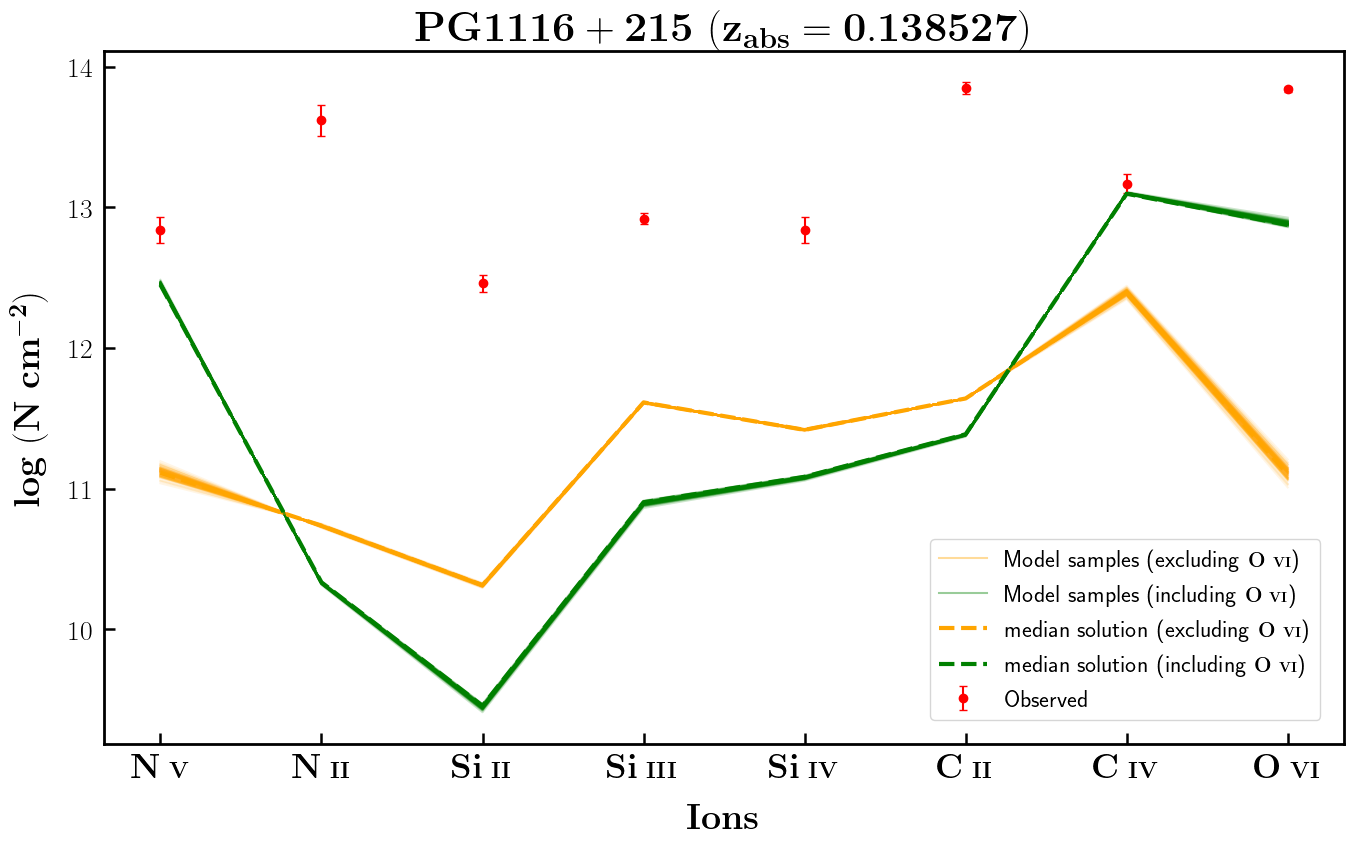
\includegraphics[width=0.85\linewidth]{Ionisation-Modelling-Plots/pg1116-z=0.138527-compII.png}
    \caption{N(\ion{H}{i})=13.60}
\end{figure}



\newpage

\begin{landscape}

\begin{figure}
    \centering
    \vspace{-20mm}
    \hspace*{-35mm}
    \captionsetup{oneside,margin={0cm,35mm}}
    \includegraphics[width=1.25\linewidth]{System-Plots/H1821+643_z=0.170006_sys_plot.png}
\end{figure}

\end{landscape}


\begin{center} 

\begin{tabular}{cccc} 

    \hline \hline \tabularnewline 
    \head{Ion} & \head{v (km s\textsuperscript{$\mathbf{-1}$})} & \head{b (km s\textsuperscript{$\mathbf{-1}$})} & \head{log [N cm\textsuperscript{$\mathbf{-2}$}]}
    \tabularnewline \tabularnewline \hline \tabularnewline 
 
    \ion{Si}{iii}   &    7 $\pm$ 3    &    17 $\pm$ 5    &     12.05 $\pm$ 0.07 \\
    \ion{Si}{iii}   &    52 $\pm$ 6    &    14 $\pm$ 10    &     11.62 $\pm$ 0.17 \\
    \ion{N}{v}   &    47 $\pm$ 3    &    31 $\pm$ 5    &     13.29 $\pm$ 0.05 \\
    \ion{N}{v}   &    122 $\pm$ 7    &    21 $\pm$ 11    &     12.74 $\pm$ 0.14 \\
    \ion{O}{vi}   &    3 $\pm$ 28    &    152 $\pm$ 20    &     13.94 $\pm$ 0.06 \\
    \ion{O}{vi}   &    107 $\pm$ 9    &    48 $\pm$ 12    &     13.29 $\pm$ 0.11 \\
    \ion{H}{i}   &    -92 $\pm$ 1    &    36 $\pm$ 1    &     13.85 $\pm$ 0.02 \\
    \ion{H}{i}   &    0 $\pm$ 2    &    63 $\pm$ 3    &     13.68 $\pm$ 0.02 \\
    \ion{H}{i}   &    120 $\pm$ 1    &    28 $\pm$ 1    &     13.35 $\pm$ 0.02 \\

    \tabularnewline \hline \hline \tabularnewline 

\end{tabular}

\end{center}

log $Z_{ref}$ = -1

N(\ion{H}{I})= 13.68  \\ 

Excluding \ion{O}{vi} : $n_H$ = -4.10 $\pm$ 0.02 \hspace{10mm} $Z$ = 0.91 $\pm$ 0.04

Including \ion{O}{vi} : $n_H$ = -4.14 $\pm$ 0.02 \hspace{10mm} $Z$ = 0.94 $\pm$ 0.04 \\

N(\ion{H}{I})= 13.35  \\ 

Excluding \ion{O}{vi} : $n_H$ = -4.07 $\pm$ 0.06 \hspace{10mm} $Z$ = 0.75 $\pm$ 0.11

Including \ion{O}{vi} : $n_H$ = -4.11 $\pm$ 0.05 \hspace{10mm} $Z$ = 0.79 $\pm$ 0.10 \\

log $Z_{ref}$ = 1

N(\ion{H}{I})= 13.68  \\ 

Excluding \ion{O}{vi} : $n_H$ = -4.33 $\pm$ 0.02 \hspace{10mm} $Z$ = 1.30 $\pm$ 0.05

Including \ion{O}{vi} : $n_H$ = -4.43 $\pm$ 0.01 \hspace{10mm} $Z$ = 1.25 $\pm$ 0.05
\\\\

N(\ion{H}{I})= 13.35  \\ 

Excluding \ion{O}{vi} : $n_H$ = -4.30 $\pm$ 0.05 \hspace{10mm} $Z$ = 1.18 $\pm$ 0.13

Including \ion{O}{vi} : $n_H$ = -4.41 $\pm$ 0.02 \hspace{10mm} $Z$ = 1.15 $\pm$ 0.12


\newpage

\begin{figure}[!h]
    \centering
    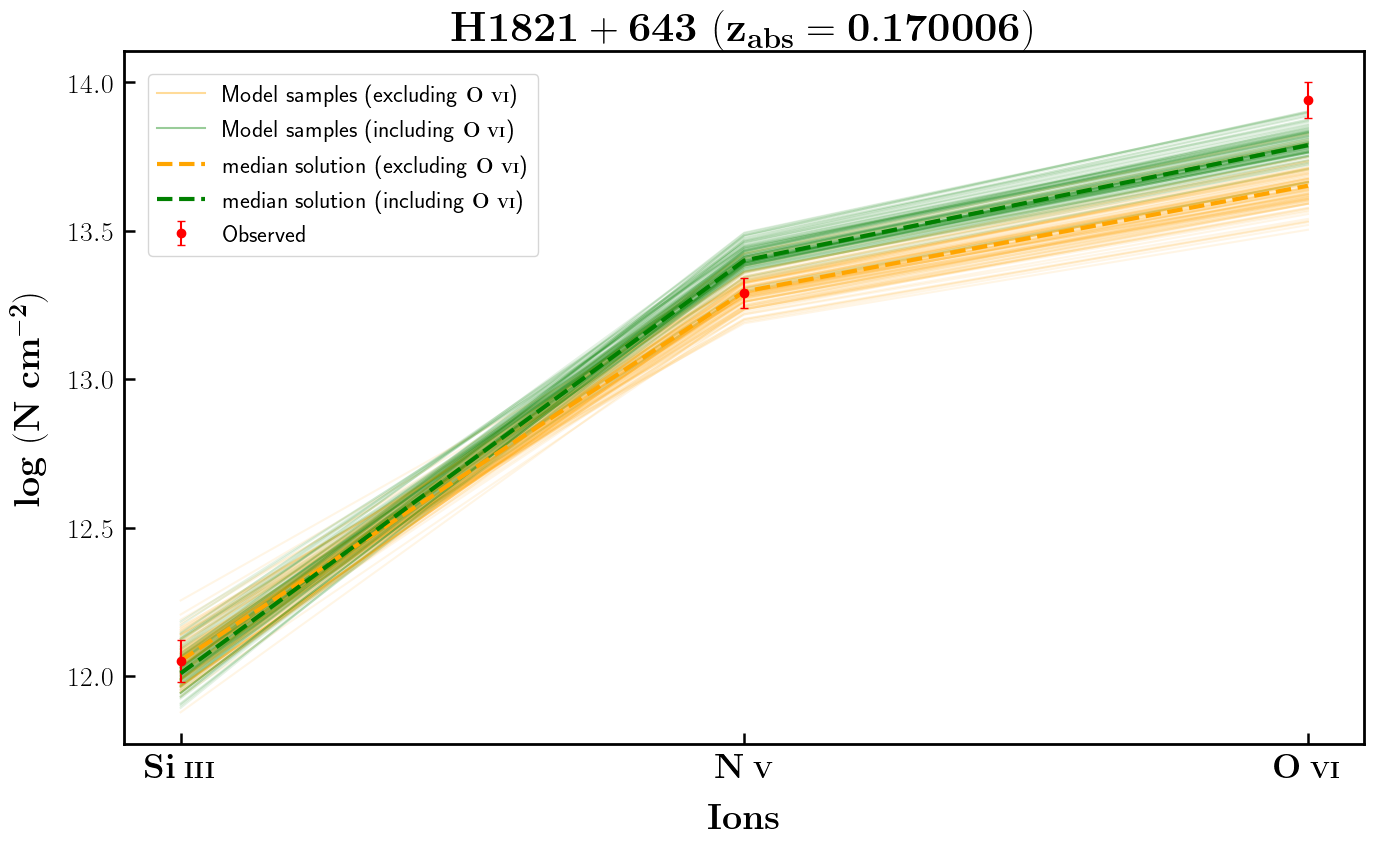
\includegraphics[width=0.85\linewidth]{Ionisation-Modelling-Plots/h1821-z=0.170006-compII_logZ=-1.png}
    \caption{N(\ion{H}{i})=13.68, log $Z_{ref}$ = -1}
\end{figure}

\begin{figure}[!b]
    \centering
    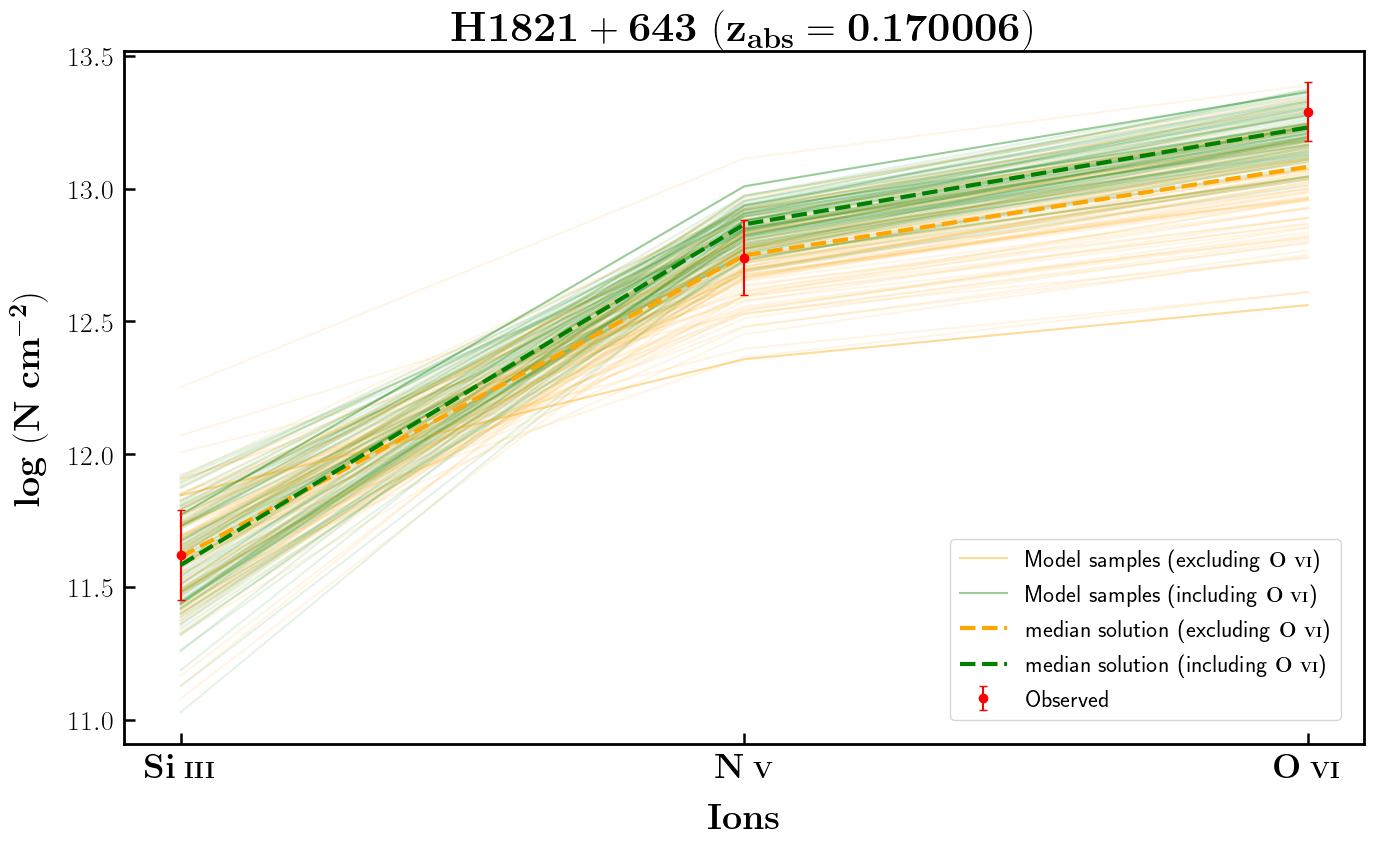
\includegraphics[width=0.85\linewidth]{Ionisation-Modelling-Plots/h1821-z=0.170006-compIII_logZ=-1.png}
    \caption{N(\ion{H}{i})=13.35, log $Z_{ref}$ = -1}
\end{figure}


\newpage

\begin{figure}[!h]
    \centering
    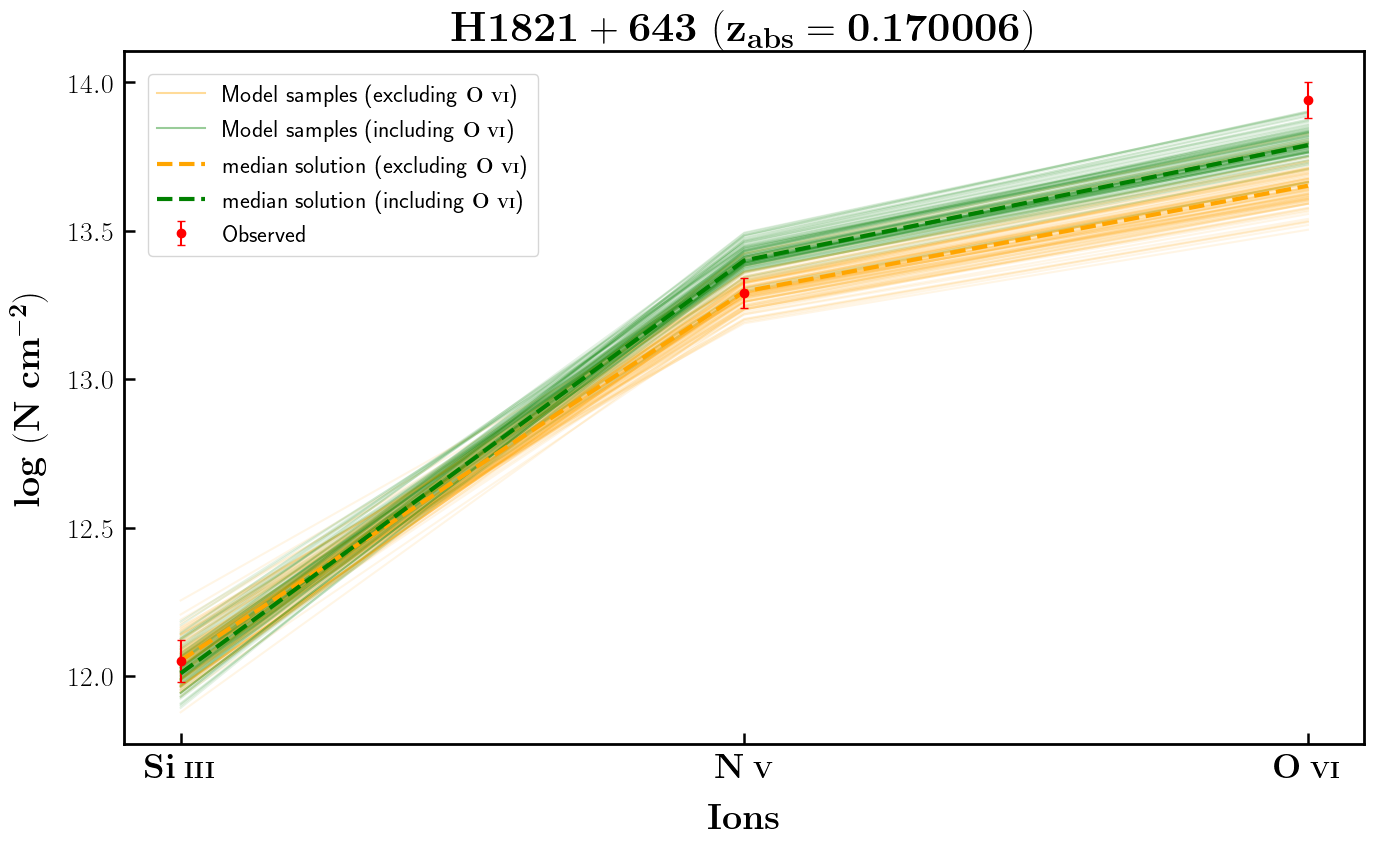
\includegraphics[width=0.85\linewidth]{Ionisation-Modelling-Plots/h1821-z=0.170006-compII.png}
    \caption{N(\ion{H}{i})=13.68, log $Z_{ref}$ = 1}
\end{figure}

\begin{figure}[!b]
    \centering
    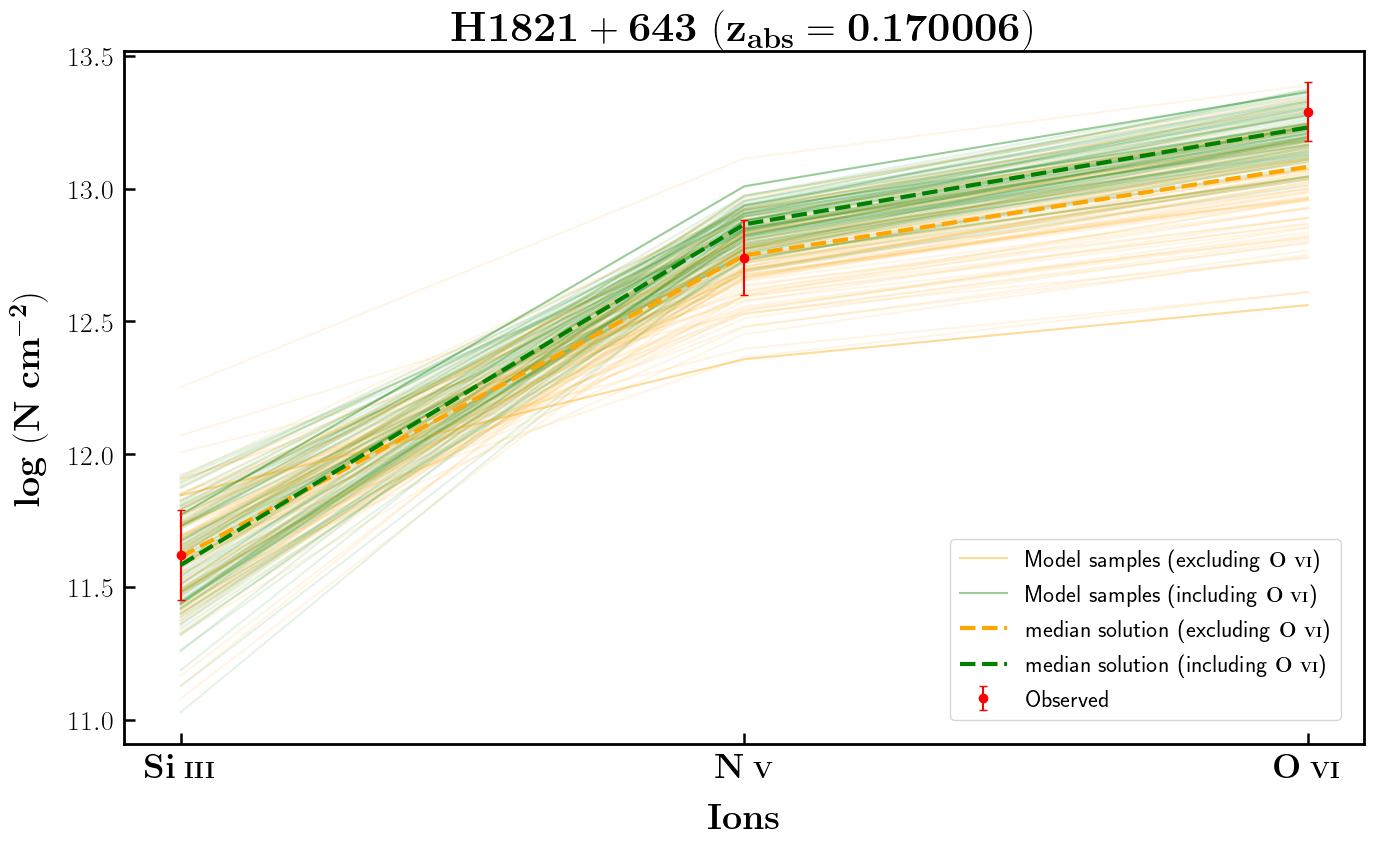
\includegraphics[width=0.85\linewidth]{Ionisation-Modelling-Plots/h1821-z=0.170006-compIII.png}
    \caption{N(\ion{H}{i})=13.35, log $Z_{ref}$ = 1}
\end{figure}



\newpage

\begin{landscape}

\begin{figure}
    \centering
    \vspace{-20mm}
    \hspace*{-35mm}
    \captionsetup{oneside,margin={0cm,35mm}}
    \includegraphics[width=1.25\linewidth]{System-Plots/H1821+643_z=0.224981_sys_plot.png}
\end{figure}

\end{landscape}


\begin{center} 

\begin{tabular}{cccc} 

    \hline \hline \tabularnewline 
    \head{Ion} & \head{v (km s\textsuperscript{$\mathbf{-1}$})} & \head{b (km s\textsuperscript{$\mathbf{-1}$})} & \head{log [N cm\textsuperscript{$\mathbf{-2}$}]}
    \tabularnewline \tabularnewline \hline \tabularnewline 
 
    \ion{Si}{iii}   &    -59 $\pm$ 13    &    31 $\pm$ 18    &     12.23 $\pm$ 0.15 \\
    \ion{Si}{iii}   &    -1 $\pm$ 6    &    22 $\pm$ 9    &     12.71 $\pm$ 0.13 \\
    \ion{C}{iii}   &    -31 $\pm$ 1    &    24 $\pm$ 2    &     13.36 $\pm$ 0.07 \\
    \ion{C}{iii}   &    12 $\pm$ 1    &    36 $\pm$ 2    &     13.84 $\pm$ 0.02 \\
    \ion{C}{iii}   &    81 $\pm$ 3    &    15 $\pm$ 5    &     12.6 $\pm$ 0.09 \\
    \ion{C}{iii}   &    335 $\pm$ 7    &    20 $\pm$ 10    &     12.13 $\pm$ 0.11 \\
    \ion{O}{vi}   &    0 $\pm$ 1    &    45 $\pm$ 1    &     14.24 $\pm$ 0.01 \\
    \ion{O}{vi}   &    57 $\pm$ 2    &    3 $\pm$ 3    &     13.12 $\pm$ 0.1 \\
    \ion{O}{vi}   &    330 $\pm$ 1    &    13 $\pm$ 2    &     13.42 $\pm$ 0.03 \\
    \ion{H}{i}   &    -109 $\pm$ 3    &    33 $\pm$ 0    &     13.87 $\pm$ 0.09 \\
    \ion{H}{i}   &    -38 $\pm$ 1    &    30 $\pm$ 1    &     15.16 $\pm$ 0.02 \\
    \ion{H}{i}   &    -19 $\pm$ 10   &    84 $\pm$ 13    &     13.64 $\pm$ 0.11 \\
    \ion{H}{i}   &    18 $\pm$ 1    &    19 $\pm$ 1    &     15.13 $\pm$ 0.03 \\
    \ion{H}{i}   &    276 $\pm$ 7    &    62 $\pm$ 11    &     13.48 $\pm$ 0.06 \\
    
    \tabularnewline \hline \hline \tabularnewline 

\end{tabular}

\end{center}


N(\ion{H}{I})= 15.16  \\ 

Excluding \ion{O}{vi} : $n_H$ = -3.29 $\pm$ 0.08 \hspace{10mm} $Z$ = -0.95 $\pm$ 0.07

Including \ion{O}{vi} : $n_H$ = -4.36 $\pm$ 0.02 \hspace{10mm} $Z$ = -0.81 $\pm$ 0.04 \\

N(\ion{H}{I})= 15.13  \\ 

Excluding \ion{O}{vi} : $n_H$ = -3.29 $\pm$ 0.03 \hspace{10mm} $Z$ = -0.44 $\pm$ 0.03

Including \ion{O}{vi} : $n_H$ = -3.83 $\pm$ 0.04 \hspace{10mm} $Z$ = -0.77 $\pm$ 0.03 \\

NOTE : Solution using $\chi^2$, MCMC didn't converge good, shows hint of two solution, another solution with high density and metallicity for both the components


\newpage

\begin{figure}[!h]
    \centering
    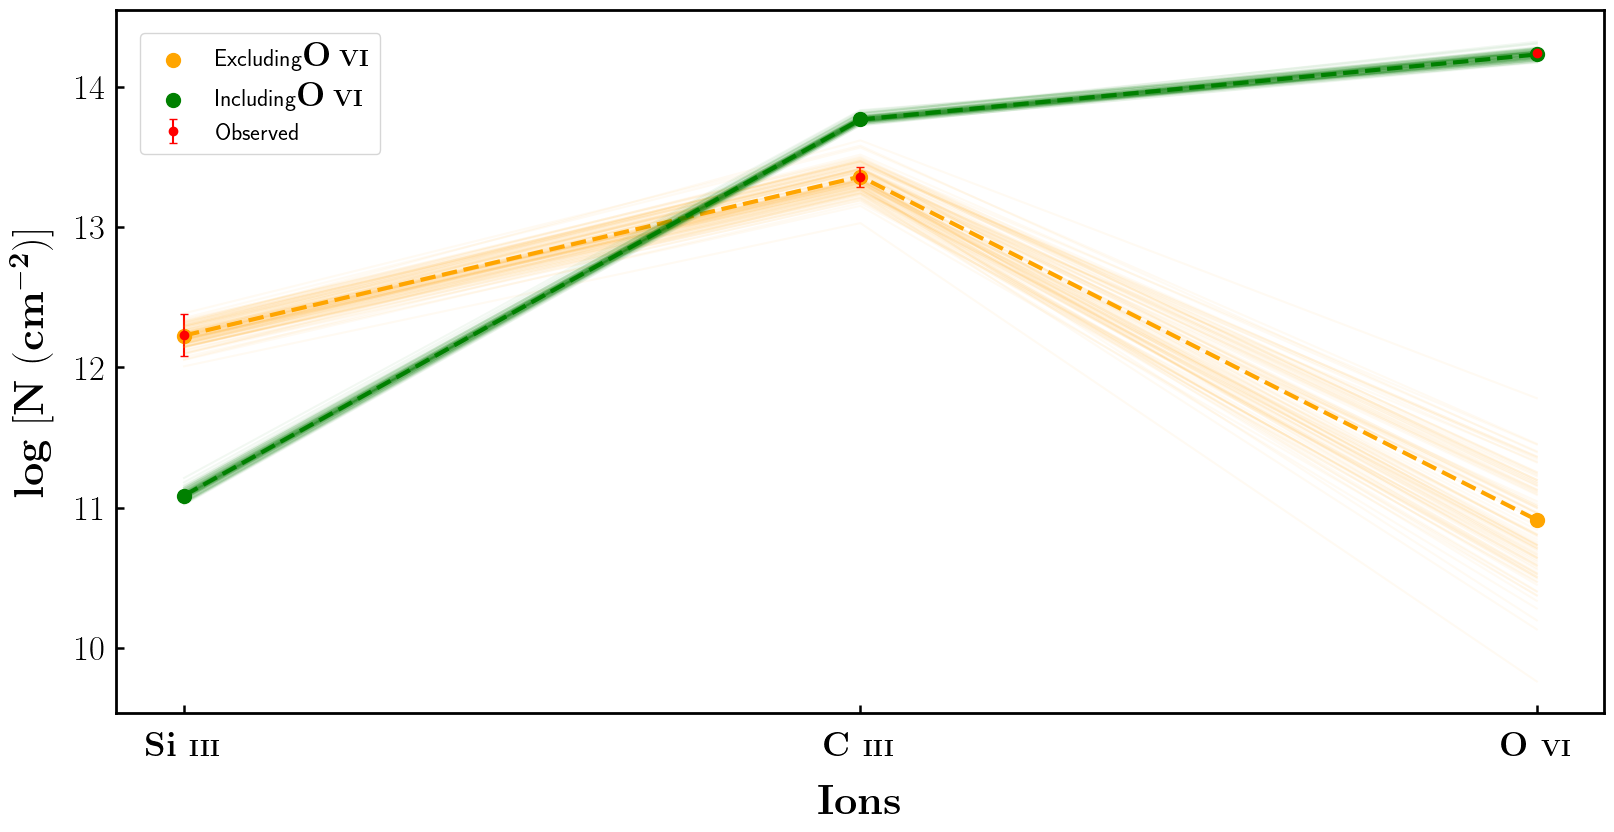
\includegraphics[width=0.85\linewidth]{Ionisation-Modelling-Plots/h1821-z=0.224981-compII.png}
    \caption{N(\ion{H}{i})=15.16}
\end{figure}

\begin{figure}[!b]
    \centering
    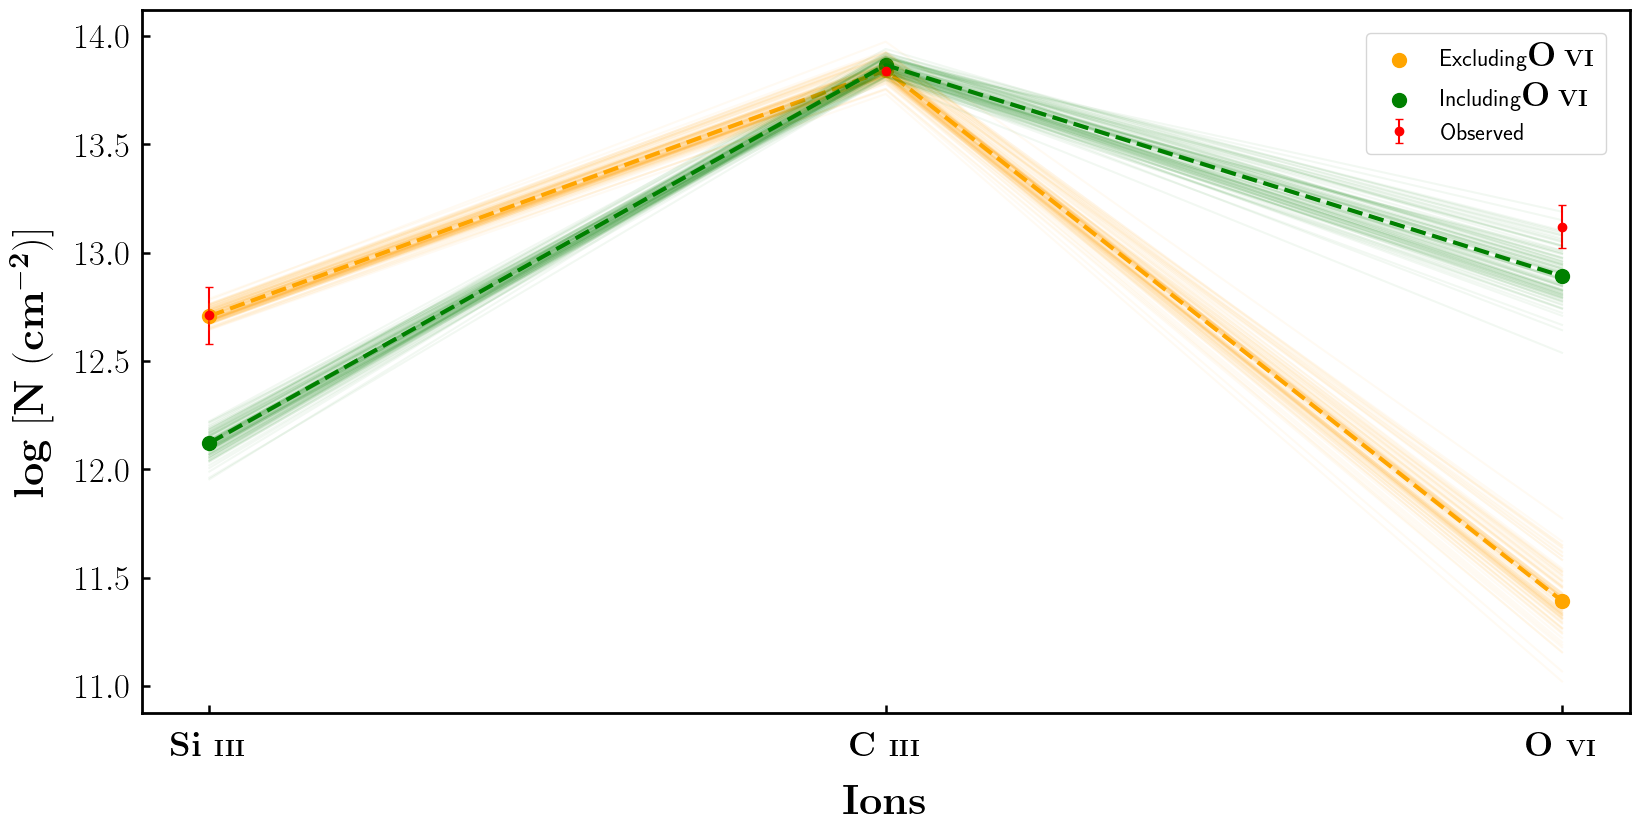
\includegraphics[width=0.85\linewidth]{Ionisation-Modelling-Plots/h1821-z=0.224981-compIV.png}
    \caption{N(\ion{H}{i})=15.13}
\end{figure}



\newpage

\begin{landscape}

\begin{figure}
    \centering
    \vspace{-20mm}
    \hspace*{-35mm}
    \captionsetup{oneside,margin={0cm,35mm}}
    \includegraphics[width=1.25\linewidth]{System-Plots/PG1121+422_z=0.192393_sys_plot.png}
\end{figure}

\end{landscape}


\begin{center} 

\begin{tabular}{cccc} 

    \hline \hline \tabularnewline 
    \head{Ion} & \head{v (km s\textsuperscript{$\mathbf{-1}$})} & \head{b (km s\textsuperscript{$\mathbf{-1}$})} & \head{log [N cm\textsuperscript{$\mathbf{-2}$}]}
    \tabularnewline \tabularnewline \hline \tabularnewline 
 
    \ion{Si}{iii}   &    -11 $\pm$ 13    &    10 $\pm$ 3    &     12.62 $\pm$ 0.10 \\
    \ion{Si}{iii}   &    9 $\pm$ 13    &    18 $\pm$ 4    &     13.14 $\pm$ 0.04 \\
    \ion{C}{iii}   &    -26 $\pm$ 10    &    10 $\pm$ 7    &     13.04 $\pm$ 0.09 \\
    \ion{C}{iii}   &    8 $\pm$ 5    &    18 $\pm$ 6    &     13.74 $\pm$ 0.11 \\
    \ion{C}{ii}   &    -9 $\pm$ 3    &    17 $\pm$ 5    &     13.69 $\pm$ 0.08 \\
    \ion{C}{ii}   &    9 $\pm$ 2    &    16 $\pm$ 3    &     13.93 $\pm$ 0.05 \\
    \ion{Si}{iv}   &    10 $\pm$ 7    &    22 $\pm$ 11    &     12.86 $\pm$ 0.13 \\
    \ion{Si}{ii}   &    -3 $\pm$ 1    &    15 $\pm$ 2    &     13.04 $\pm$ 0.06 \\
    \ion{Si}{ii}   &    27 $\pm$ 19    &    42 $\pm$ 1    &     12.48 $\pm$ 0.23 \\
    \ion{O}{vi}   &    -7 $\pm$ 13    &    11 $\pm$ 16    &     12.84 $\pm$ 0.19 \\
    \ion{O}{vi}   &    20 $\pm$ 3    &    3 $\pm$ 4    &     13.37 $\pm$ 0.12 \\
    \ion{H}{i}   &    1 $\pm$ 2    &    60 $\pm$ 6    &     14.34 $\pm$ 0.09 \\
    \ion{H}{i}   &    5 $\pm$ 1    &    19 $\pm$ 1    &     17.7 $\pm$ 0.11 \\

    \tabularnewline \hline \hline \tabularnewline 

\end{tabular}

\end{center}


N(\ion{H}{I})=14.34   \\ 

log $Z_{ref}$ = -1

Excluding \ion{O}{vi} : $n_H$ = -1.78 $\pm$ 0.05 \hspace{10mm} $Z$ = 1.97 $\pm$ 0.04

Including \ion{O}{vi} : $n_H$ = -3.00 $\pm$ 0.04 \hspace{10mm} $Z$ = 1.25 $\pm$ 0.04 \\

log $Z_{ref}$ = 1 

Excluding \ion{O}{vi} : $n_H$ = -3.12 $\pm$ 0.07 \hspace{10mm} $Z$ = 1.62 $\pm$ 0.07

Including \ion{O}{vi} : $n_H$ = -3.7 $\pm$ 0.03 \hspace{10mm} $Z$ = 1.33 $\pm$ 0.04 \\\\

N(\ion{H}{I})= 17.70  

Excluding \ion{O}{vi} : $n_H$ = -2.35 $\pm$ 0.05 \hspace{10mm} $Z$ = -1.66 $\pm$ 0.06

Including \ion{O}{vi} : $n_H$ = -3.08 $\pm$ 0.04 \hspace{10mm} $Z$ = -2.08 $\pm$ 0.05 \\

NOTE : Since very high N(\ion{H}{i}), so low metallicity. And solutions aren't much good.


\newpage

\begin{figure}[!h]
    \centering
    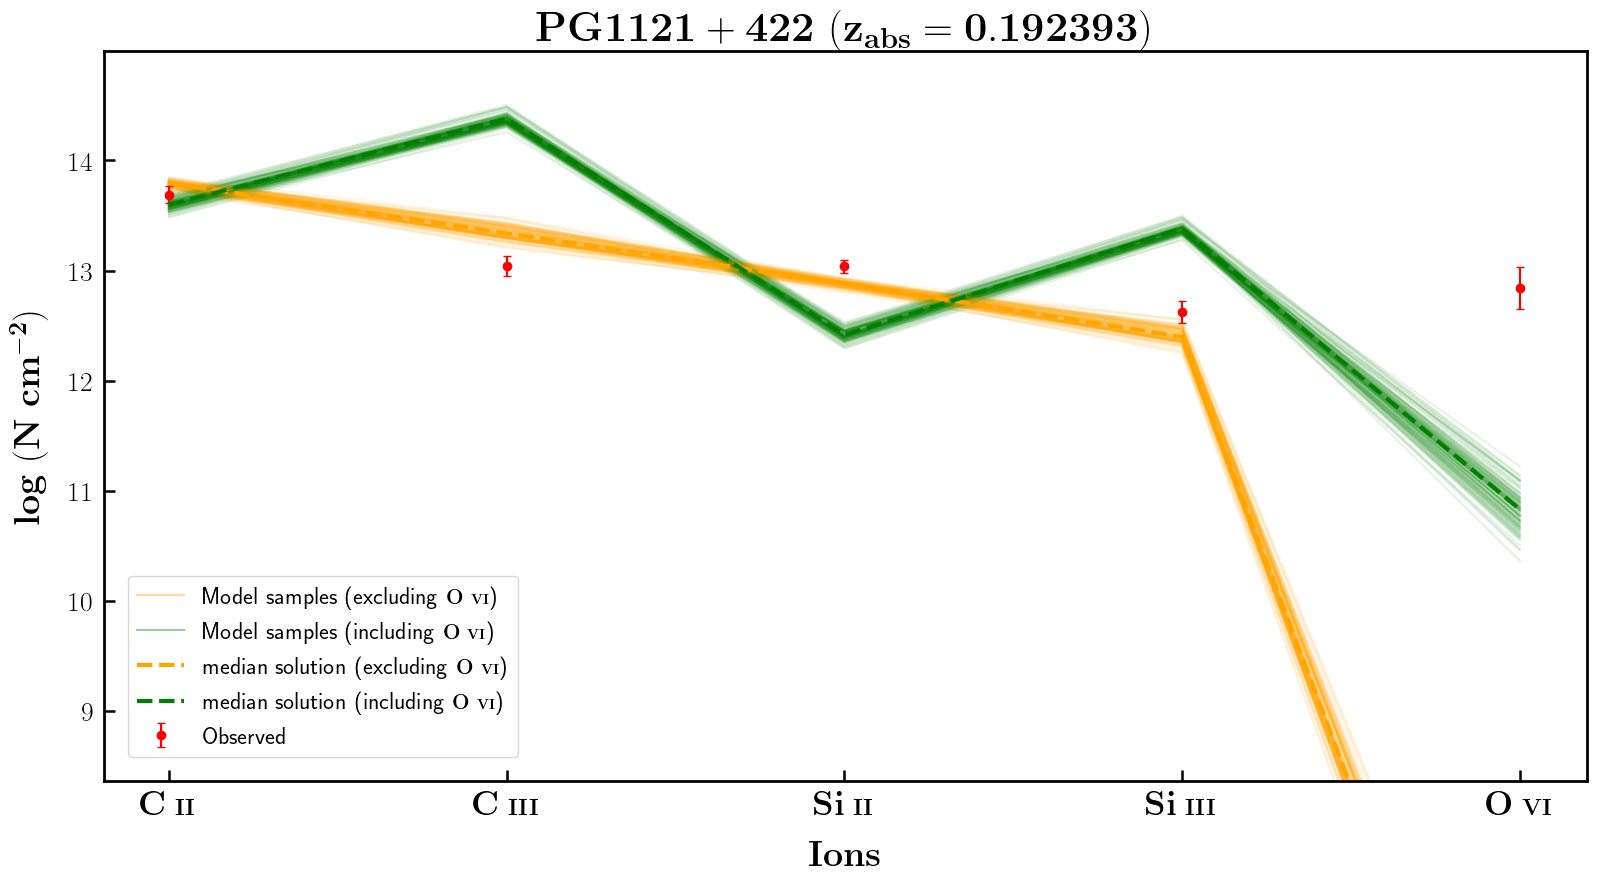
\includegraphics[width=0.85\linewidth]{Ionisation-Modelling-Plots/pg1121-z=0.192393-compI_logZ=-1.png}
    \caption{N(\ion{H}{i})=14.34, log $Z_{ref}$=-1}
\end{figure}

\begin{figure}[!b]
    \centering
    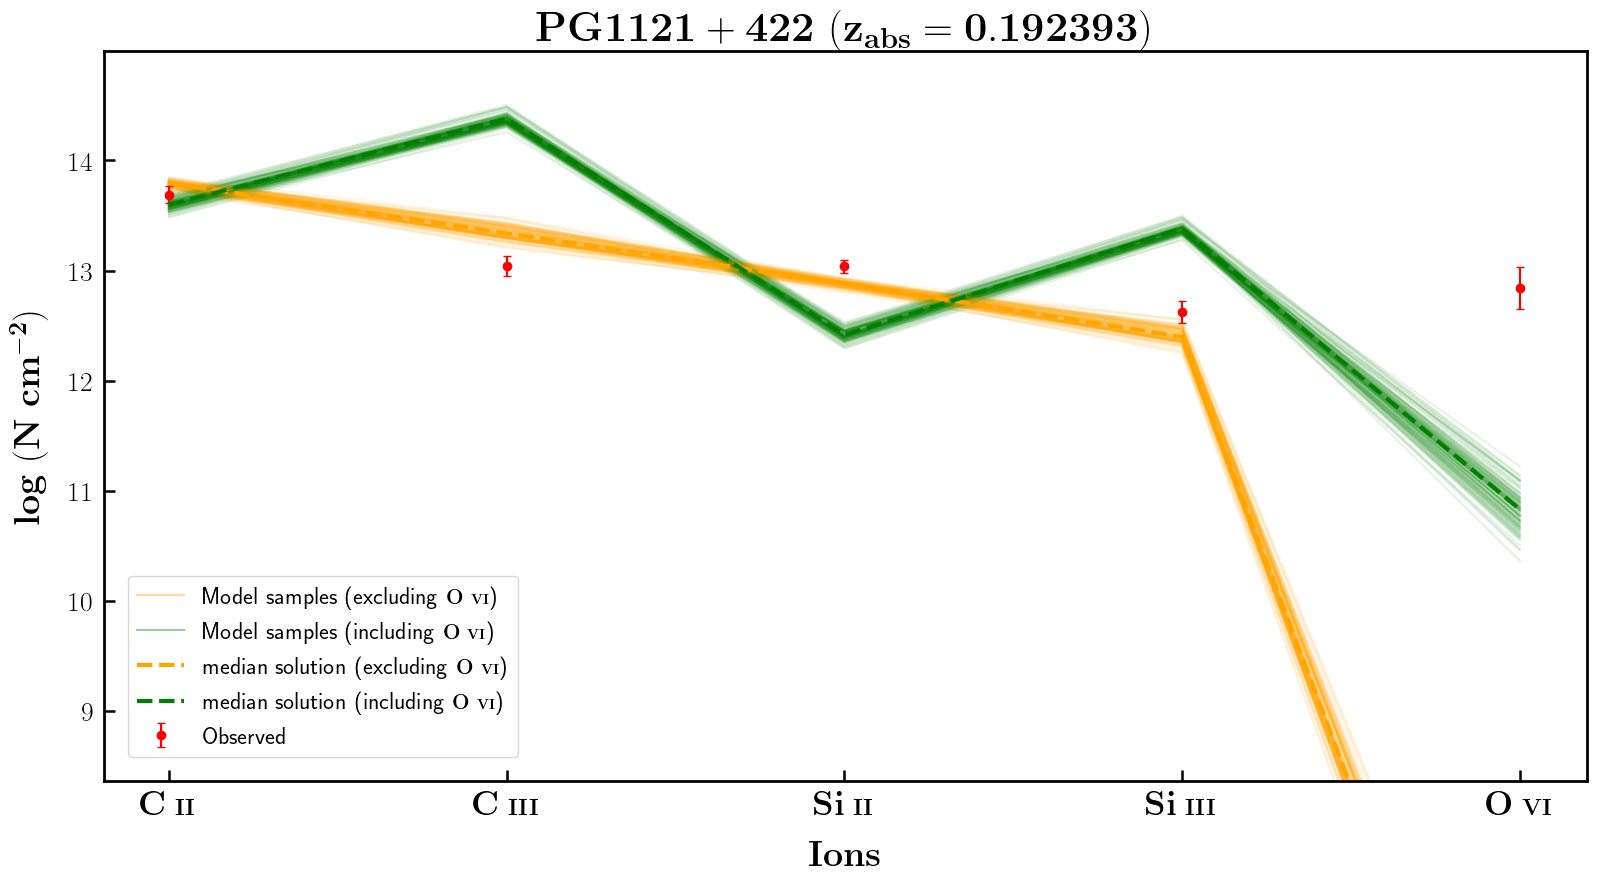
\includegraphics[width=0.85\linewidth]{Ionisation-Modelling-Plots/pg1121-z=0.192393-compI.png}
    \caption{N(\ion{H}{i})=14.34, log $Z_{ref}$=1}
\end{figure}

\begin{figure}[!t]
    \centering
    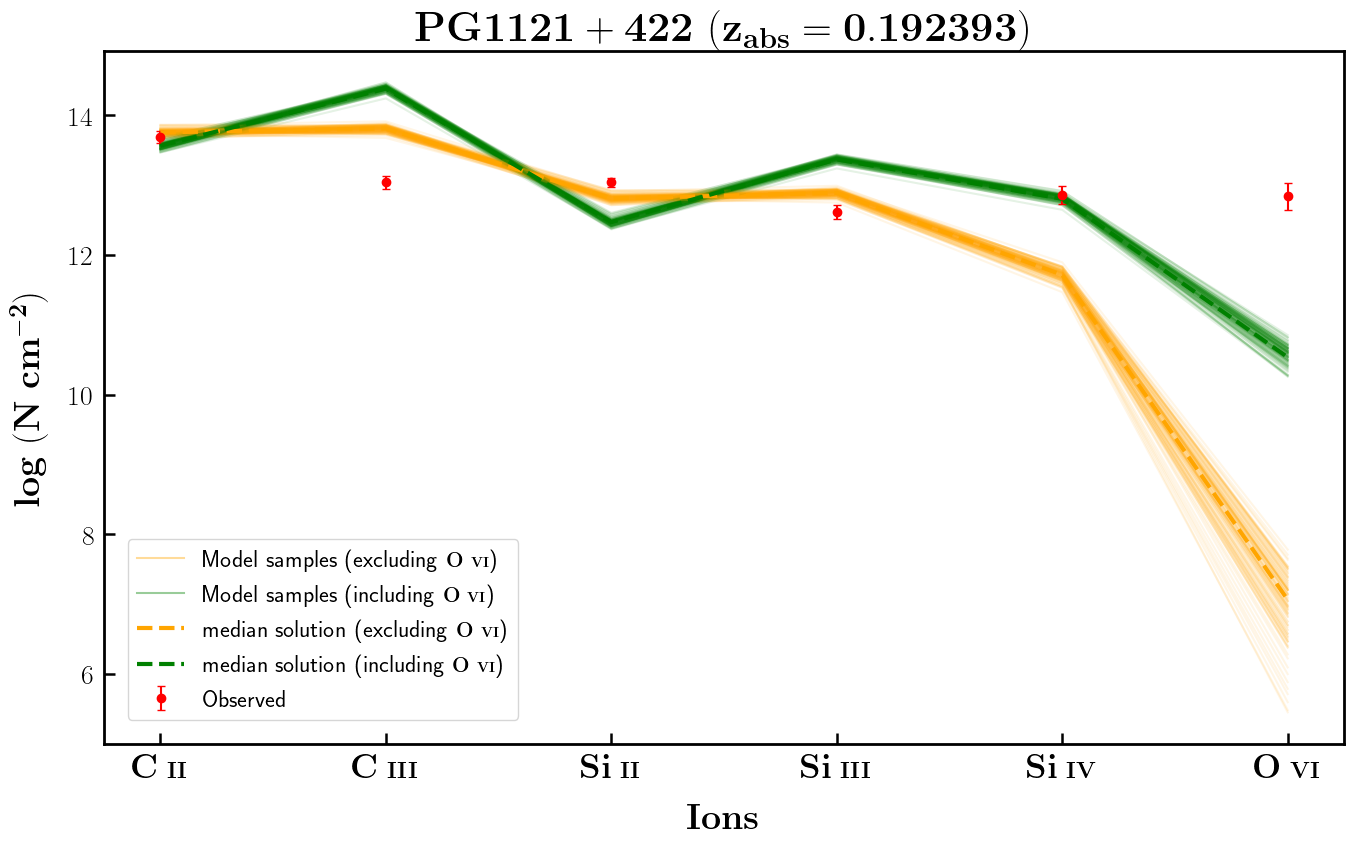
\includegraphics[width=0.85\linewidth]{Ionisation-Modelling-Plots/pg1121-z=0.192393-compII.png}
    \caption{N(\ion{H}{i})=17.70, log $Z_{ref}$=-1}
\end{figure}








\newpage

\begin{landscape}

\begin{figure}
    \centering
    \vspace{-20mm}
    \hspace*{-35mm}
    \captionsetup{oneside,margin={0cm,35mm}}
    \includegraphics[width=1.25\linewidth]{System-Plots/PKS0405-123_z=0.167125_sys_plot.png}
\end{figure}

\end{landscape}


\begin{center} 

\begin{tabular}{cccc} 

    \hline \hline \tabularnewline 
    \head{Ion} & \head{v (km s\textsuperscript{$\mathbf{-1}$})} & \head{b (km s\textsuperscript{$\mathbf{-1}$})} & \head{log [N cm\textsuperscript{$\mathbf{-2}$}]}
    \tabularnewline \tabularnewline \hline \tabularnewline 
 
    \ion{O}{i}   &    -14 $\pm$ 5    &    23 $\pm$ 7    &     13.52 $\pm$ 0.08 \\
    \ion{C}{ii}   &    -37 $\pm$ 2    &    16 $\pm$ 2    &     13.76 $\pm$ 0.02 \\
    \ion{C}{ii}   &    -1 $\pm$ 1    &    6 $\pm$ 1    &     16.27 $\pm$ 0.12 \\
    \ion{C}{iii}   &    -136 $\pm$ 2    &    32 $\pm$ 2    &     13.45 $\pm$ 0.02 \\
    \ion{C}{iii}   &    -26 $\pm$ 0    &    37 $\pm$ 2    &     14.33 $\pm$ 0.04 \\
    \ion{N}{ii}   &    -27 $\pm$ 6    &    44 $\pm$ 5    &     13.47 $\pm$ 0.09 \\
    \ion{N}{ii}   &    -7 $\pm$ 1    &    12 $\pm$ 1    &     14.11 $\pm$ 0.02 \\
    \ion{N}{iii}   &    -7 $\pm$ 0    &    9 $\pm$ 4    &     14.06 $\pm$ 0.08 \\
    \ion{N}{iii}   &    5 $\pm$ 0    &    50 $\pm$ 2    &     14.43 $\pm$ 0.02 \\
    \ion{N}{v}   &    -276 $\pm$ 3    &    30 $\pm$ 0    &     13.25 $\pm$ 0.05 \\
    \ion{N}{v}   &    -116 $\pm$ 0    &    59 $\pm$ 9    &     13.32 $\pm$ 0.08 \\
    \ion{N}{v}   &    -79 $\pm$ 13    &    24 $\pm$ 12    &     12.77 $\pm$ 0.19 \\
    \ion{N}{v}   &    -3 $\pm$ 2    &    43 $\pm$ 3    &     13.89 $\pm$ 0.03 \\
    \ion{Si}{iii}   &    -41 $\pm$ 3    &    13 $\pm$ 4    &     12.66 $\pm$ 0.10 \\
    \ion{Si}{iii}   &    -1 $\pm$ 2    &    22 $\pm$ 2    &     13.28 $\pm$ 0.03 \\
    \ion{Si}{iv}   &    -128 $\pm$ 0    &    25 $\pm$ 5    &     12.61 $\pm$ 0.06 \\
    \ion{Si}{iv}   &    2 $\pm$ 1    &    31 $\pm$ 2    &     13.25 $\pm$ 0.02 \\
    \ion{Si}{ii}   &    -48 $\pm$ 5    &    26 $\pm$ 8    &     12.54 $\pm$ 0.09 \\
    \ion{Si}{ii}   &    -4 $\pm$ 1    &    15 $\pm$ 0    &     13.24 $\pm$ 0.02 \\
    \ion{O}{vi}   &    -268 $\pm$ 0    &    74 $\pm$ 5    &     14.05 $\pm$ 0.02 \\
    \ion{O}{vi}   &    -129 $\pm$ 8    &    41 $\pm$ 3    &     14.05 $\pm$ 0.10 \\
    \ion{O}{vi}   &    -64 $\pm$ 5    &    32 $\pm$ 2    &     14.11 $\pm$ 0.17 \\
    \ion{O}{vi}   &    -2 $\pm$ 4    &    43 $\pm$ 3    &     14.49 $\pm$ 0.05 \\
    \ion{H}{i}   &    -158 $\pm$ 0    &    56 $\pm$ 9    &     13.09 $\pm$ 0.06 \\
    \ion{H}{i}   &    -127 $\pm$ 4    &    26 $\pm$ 3    &     13.46 $\pm$ 0.04 \\
    \ion{H}{i}   &    -80 $\pm$ 1    &    18 $\pm$ 2    &     13.54 $\pm$ 0.04 \\
    \ion{H}{i}   &    -30 $\pm$ 0    &    18 $\pm$ 2    &     15.98 $\pm$ 0.34 \\
    \ion{H}{i}   &    8 $\pm$ 49    &    19 $\pm$ 0    &     17.53 $\pm$ 0.07 \\
    \ion{H}{i}   &    54 $\pm$ 90    &    30 $\pm$ 2    &     13.66 $\pm$ 0.04 \\
    
    \tabularnewline \hline \hline \tabularnewline 

\end{tabular}

\end{center}


N(\ion{H}{I})= 13.46  \\ 

Excluding \ion{O}{vi} : $n_H$ = -3.98 $\pm$ 0.03 \hspace{10mm} $Z$ = 0.62 $\pm$ 0.02

Including \ion{O}{vi} : $n_H$ = -4.17 $\pm$ 0.02 \hspace{10mm} $Z$ = 0.63 $\pm$ 0.02
\\\\

N(\ion{H}{I})= 15.98  \\ 

Excluding \ion{O}{vi} : $n_H$ = -2.73 $\pm$ 0.04 \hspace{10mm} $Z$ = -0.18 $\pm$ 0.02

Including \ion{O}{vi} : $n_H$ = -3.27 $\pm$ 0.03 \hspace{10mm} $Z$ = -0.33 $\pm$ 0.02
\\\\



\newpage

\begin{figure}[!h]
    \centering
    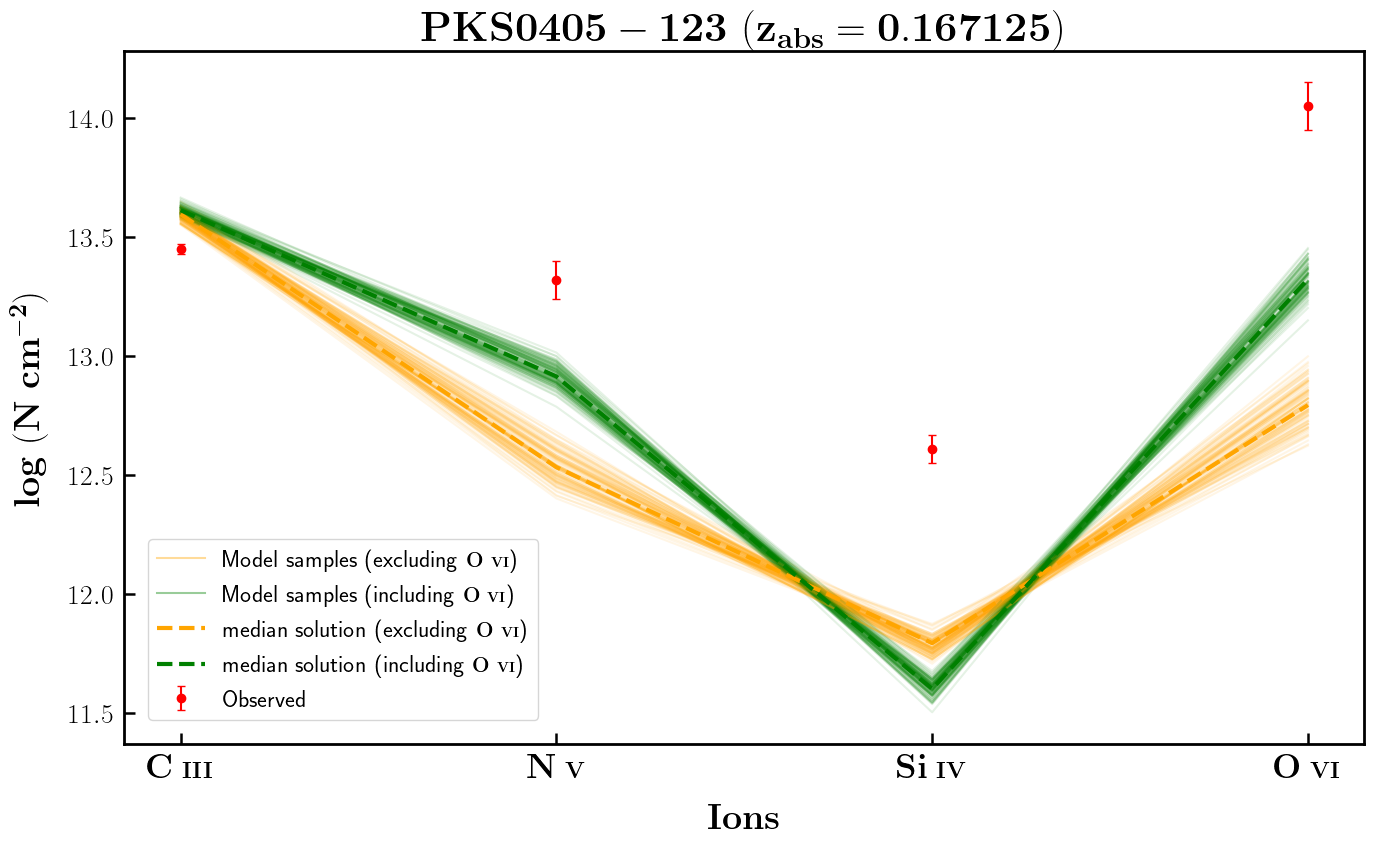
\includegraphics[width=0.85\linewidth]{Ionisation-Modelling-Plots/pks0405-z=0.167125-compII.png}
    \caption{N(\ion{H}{i})=13.46}
\end{figure}

\begin{figure}[!b]
    \centering
    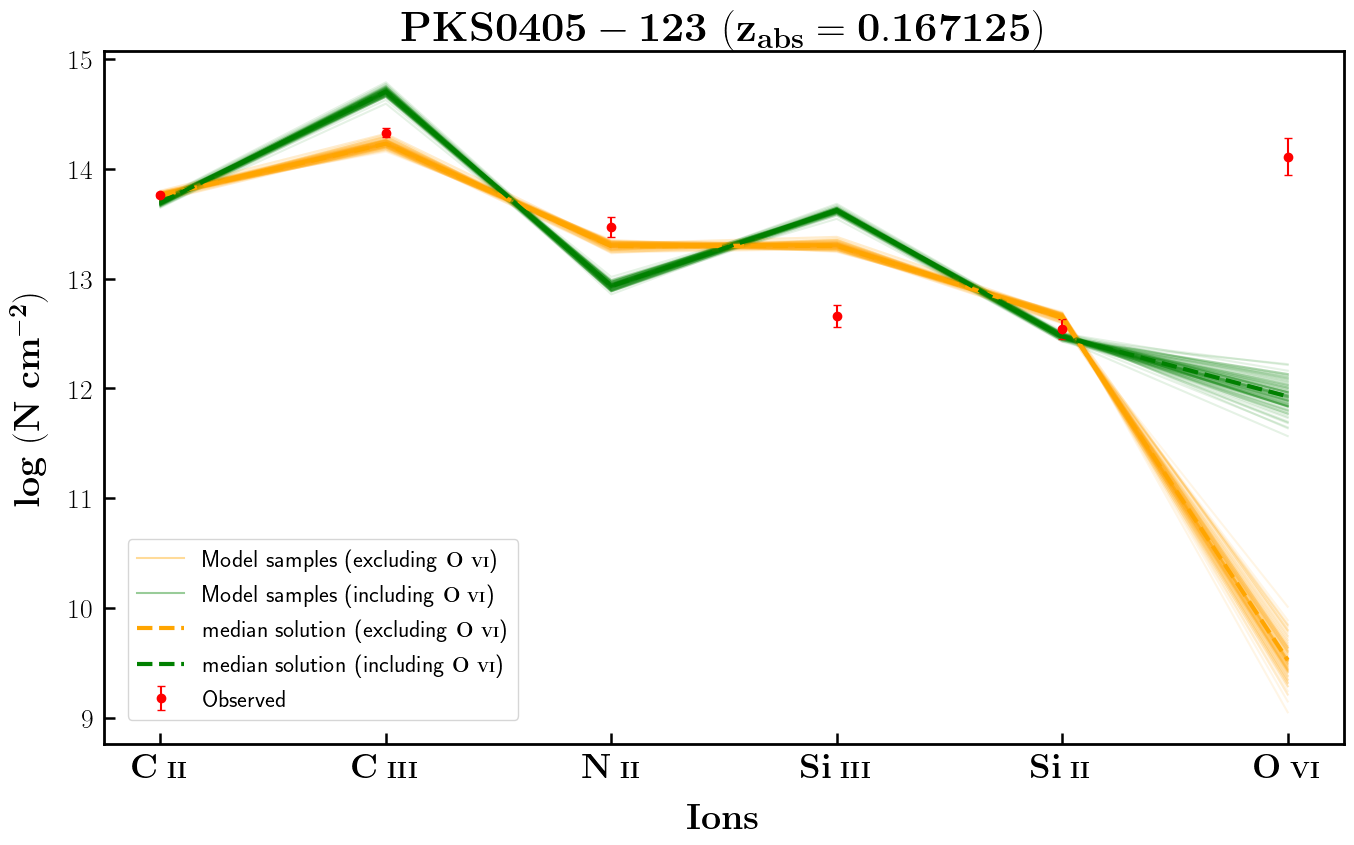
\includegraphics[width=0.85\linewidth]{Ionisation-Modelling-Plots/pks0405-z=0.167125-compIV.png}
    \caption{N(\ion{H}{i})=15.98}
\end{figure}




\end{document}

